\section{Preventivo}
In questa sezione del documento viene riportata la distribuzione delle risorse del gruppo nei vari periodi di svolgimento del progetto.\\
Inoltre sono illustrate la pianificazione e distribuzione oraria dei ruoli per ogni membro del gruppo, i quali devono:
\begin{itemize}
	\item Ricoprire tutti i ruoli durante tutta la durata del progetto;
	\item Avere circa le stesse ore produttive alla fine di ogni periodo del progetto.
\end{itemize}
Inoltre il verificatore di un determinato task\textsubscript{G} non potrà essere colui che lo ha svolto.\\
Il riferimento alle sigle identificative dei ruoli si può trovare al paragrafo 3.1.5.5 del documento \textit{Norme di progetto v1.0.0}.
\newpage
\subsection{Analisi}
%
% ----------------------------------------------------------------------------------------------------------------
\subsubsection{Sprint\textsubscript{G} I}
% ----------------------------------------------------------------------------------------------------------------
%
\subsubsubsection{Preventivo orario}
La seguente tabella rappresenta la distribuzione oraria di ogni membro del gruppo per il primo sprint\textsubscript{G} del progetto, il quale è svolto nel periodo di analisi:

	\setlength\extrarowheight{5pt}
	\rowcolors{2}{gray!10}{gray!40}
	\begin{tabularx}{\textwidth}{|ccccccc|c|}
		\hline
		\rowcolor{white}
		\textbf{Nome} & \textbf{Re} & \textbf{Am} & \textbf{An} & \textbf{Ve} & \textbf{Pr}& \textbf{Pt} & \textbf{Ore totali} \\
		\hline
		Nicola Sinicato &3&3&4&0&0&0&10 \\
		Gabriele Da Re &0&6&4&0&0&0&10 \\
		Luca Brugnera &0&6&4&0&0&0&10 \\
		Matteo Stocco &1&5&4&0&0&0&10 \\
		Ana Lazic &1&3&6&0&0&0&10 \\
		Zhen Wei Zheng &1&3&6&0&0&0&10 \\
		\hline
		Ore totali ruolo &6&26&28&0&0&0&60 \\
		\hline
		\rowcolor{white}
		\caption{Distribuzione oraria durante il primo sprint\textsubscript{G} per ruolo e persona}
	\end{tabularx}
	\vspace{10pt}
	

\begin{figure}[H]
    \centering
    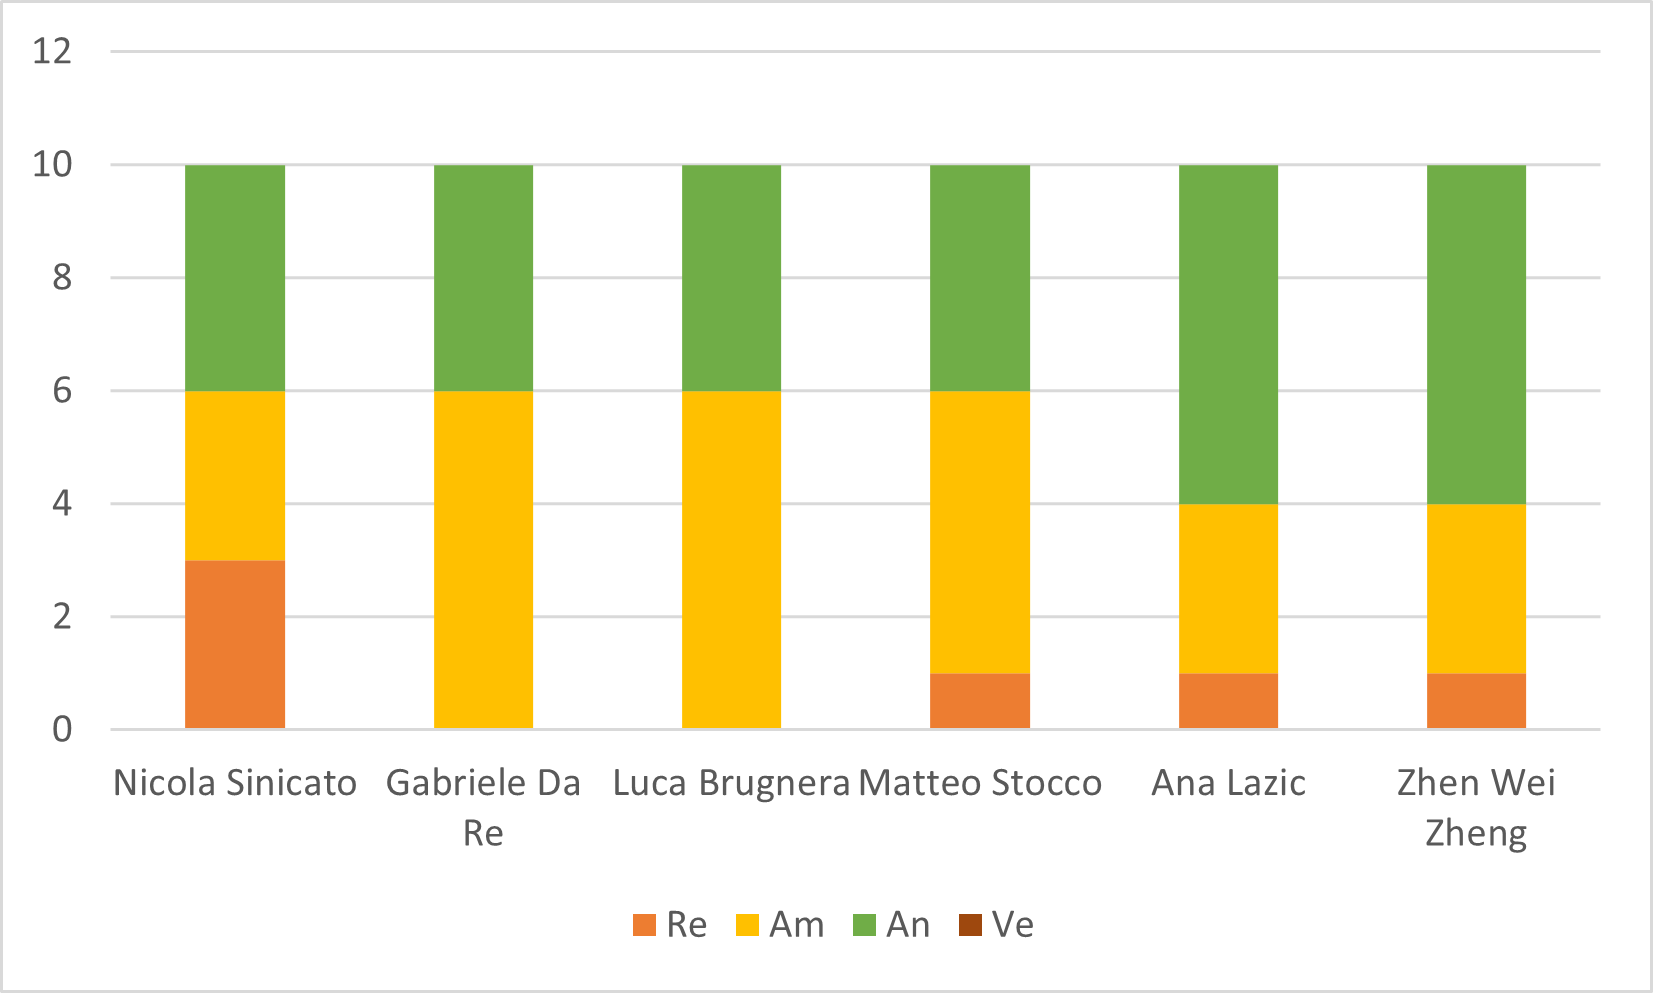
\includegraphics[scale=0.6]{img/grafi preventivo/istogrammi/analisi/sprint1.png}
    \caption{Istogramma con la ripartizione delle ore del primo sprint\textsubscript{G}}
\end{figure}
\begin{figure}[H]
    \centering
    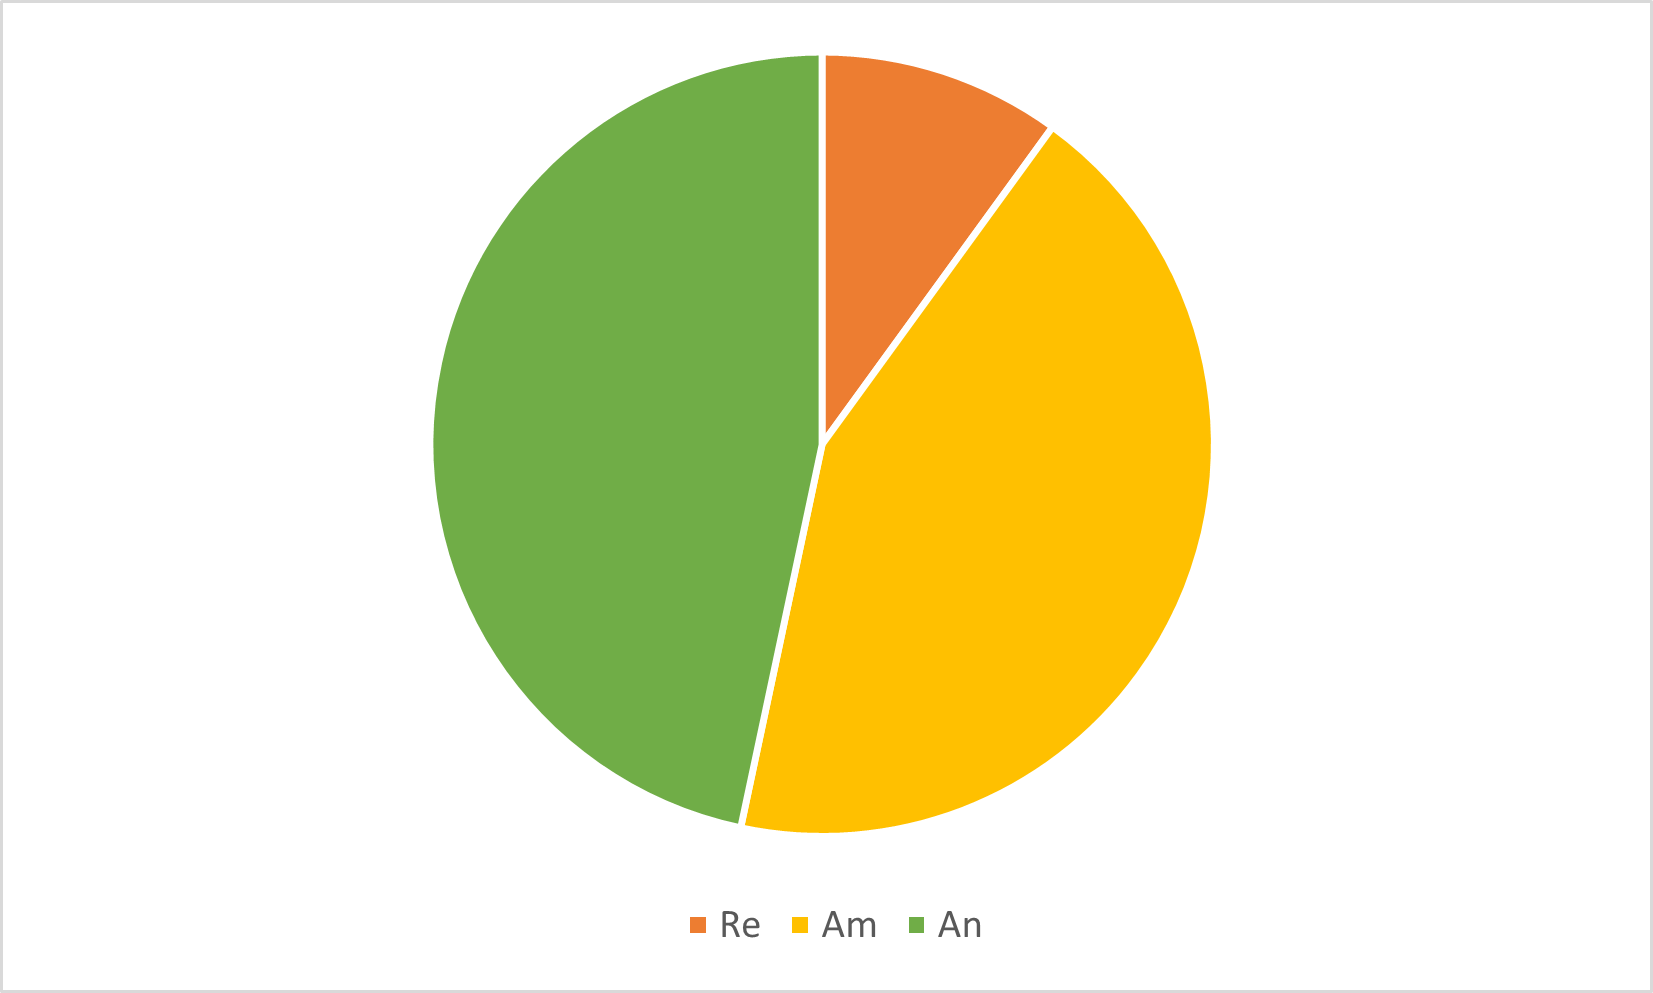
\includegraphics[scale=0.6]{img/grafi preventivo/torta/analisi/sprint1.png}
    \caption{Grafico a torta con la ripartizione delle ore per ruolo nel primo sprint\textsubscript{G}}
\end{figure}

\subsubsubsection{Preventivo dei costi}
La seguente tabella rappresenta le ore dedicate ad ogni ruolo e il corrispettivo costo in euro per il primo sprint\textsubscript{G}, svolto nel periodo di analisi:

	\setlength\extrarowheight{5pt}
	\rowcolors{2}{gray!10}{gray!40}
	\begin{tabularx}{\textwidth}{|ccc|c|}
		\hline
		\rowcolor{white}
		\textbf{Ruolo} & \textbf{Costo orario (€)} & \textbf{Ore totali} & \textbf{Costo totale (€)} \\
		\hline
		Responsabile &30&6&180 \\
		Amministratore &20&26&520 \\
		Analista &25&28&700 \\
		Verificatore &15&0&0 \\
		Programmatore &15&0&0 \\
		Progettista &25&0&0 \\
		\hline
		Totale &-&-&1400 \\
		\hline
		\rowcolor{white}
		\caption{Prospetto del costo orario durante il primo sprint\textsubscript{G} per ruolo}
	\end{tabularx}
    \vspace{10pt}
	
% ----------------------------------------------------------------------------------------------------------------
\newpage
\subsubsection{Sprint\textsubscript{G} II}
% ----------------------------------------------------------------------------------------------------------------
%
\subsubsubsection{Preventivo orario}
La seguente tabella rappresenta la distribuzione oraria di ogni membro del gruppo per il secondo sprint\textsubscript{G} del progetto, il quale è svolto nel periodo di analisi:

	\setlength\extrarowheight{5pt}
	\rowcolors{2}{gray!10}{gray!40}
	\begin{tabularx}{\textwidth}{|ccccccc|c|}
		\hline
		\rowcolor{white}
		\textbf{Nome} & \textbf{Re} & \textbf{Am} & \textbf{An} & \textbf{Ve} & \textbf{Pr}& \textbf{Pt} & \textbf{Ore totali} \\
		\hline
		Nicola Sinicato &2&1&8&4&0&0&15 \\
		Gabriele Da Re &1&4&7&3&0&0&15 \\
		Luca Brugnera &1&5&6&3&0&0&15 \\
		Matteo Stocco &2&2&7&4&0&0&15 \\
		Ana Lazic &0&2&7&6&0&0&15 \\
		Zhen Wei Zheng &0&2&6&7&0&0&15 \\
		\hline
		Ore totali ruolo &6&16&41&27&0&0&90 \\
		\hline
		\rowcolor{white}
		\caption{Distribuzione oraria durante il secondo sprint\textsubscript{G} per ruolo e persona}
	\end{tabularx}
	\vspace{10pt}
	
\begin{figure}[H]
    \centering
    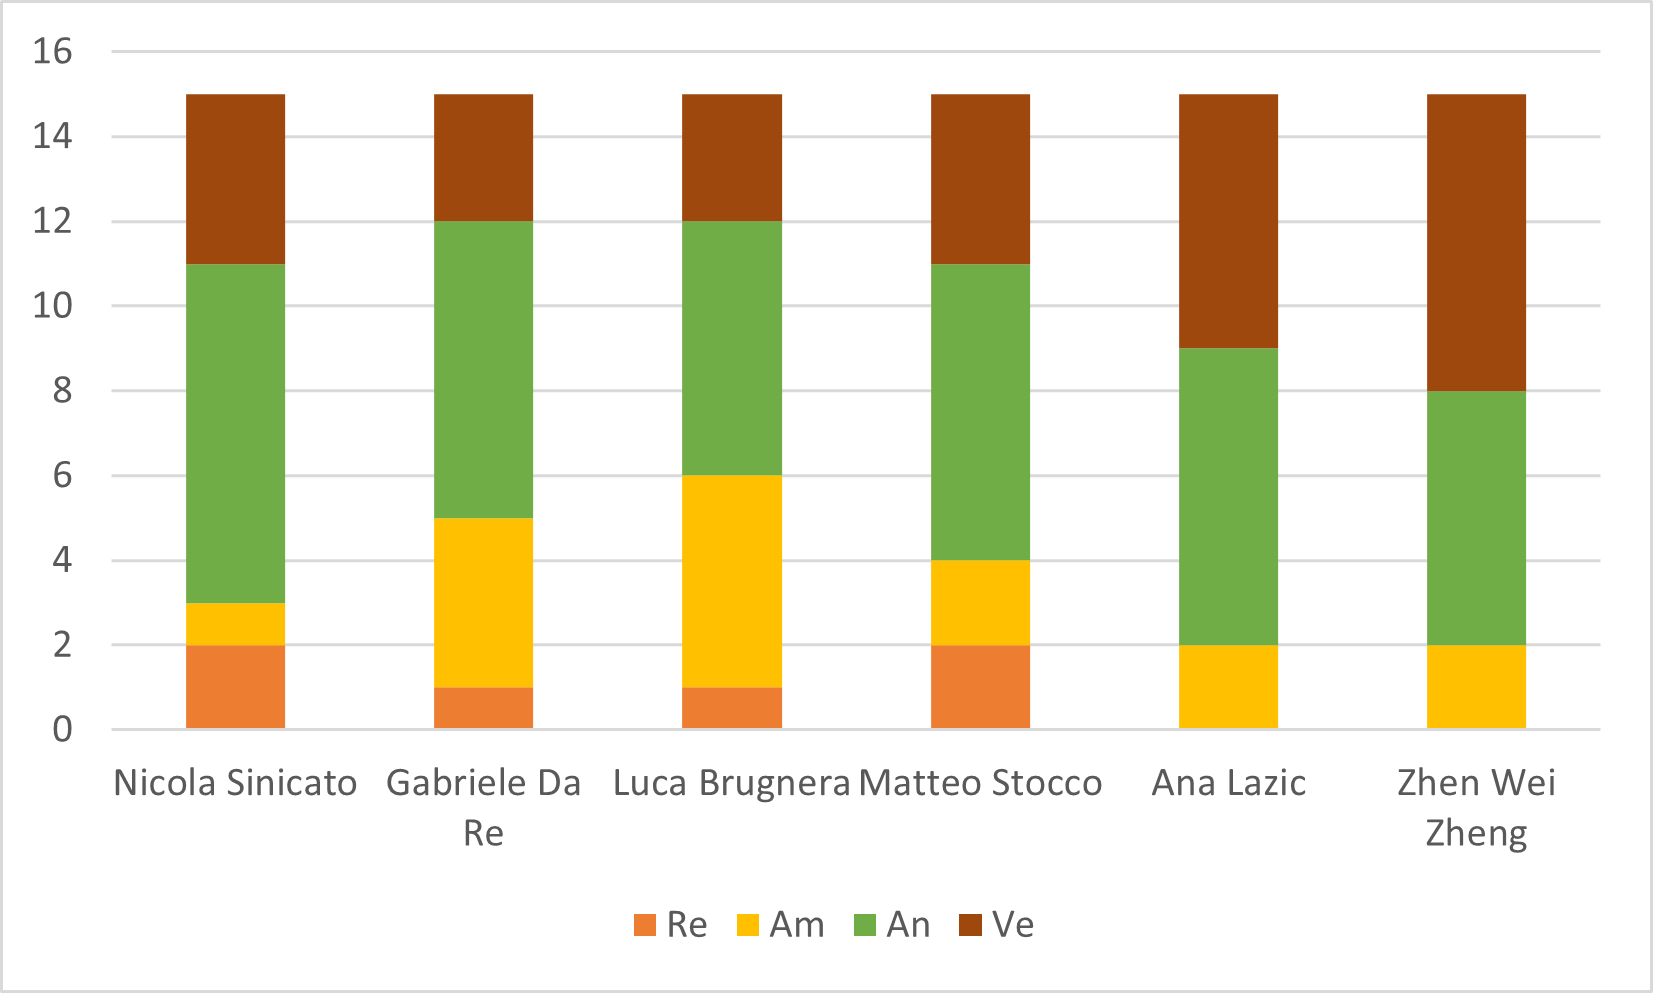
\includegraphics[scale=0.6]{img/grafi preventivo/istogrammi/analisi/sprint2.png}
    \caption{Istogramma con la ripartizione delle ore del secondo sprint\textsubscript{G}}
\end{figure}
\begin{figure}[H]
    \centering
    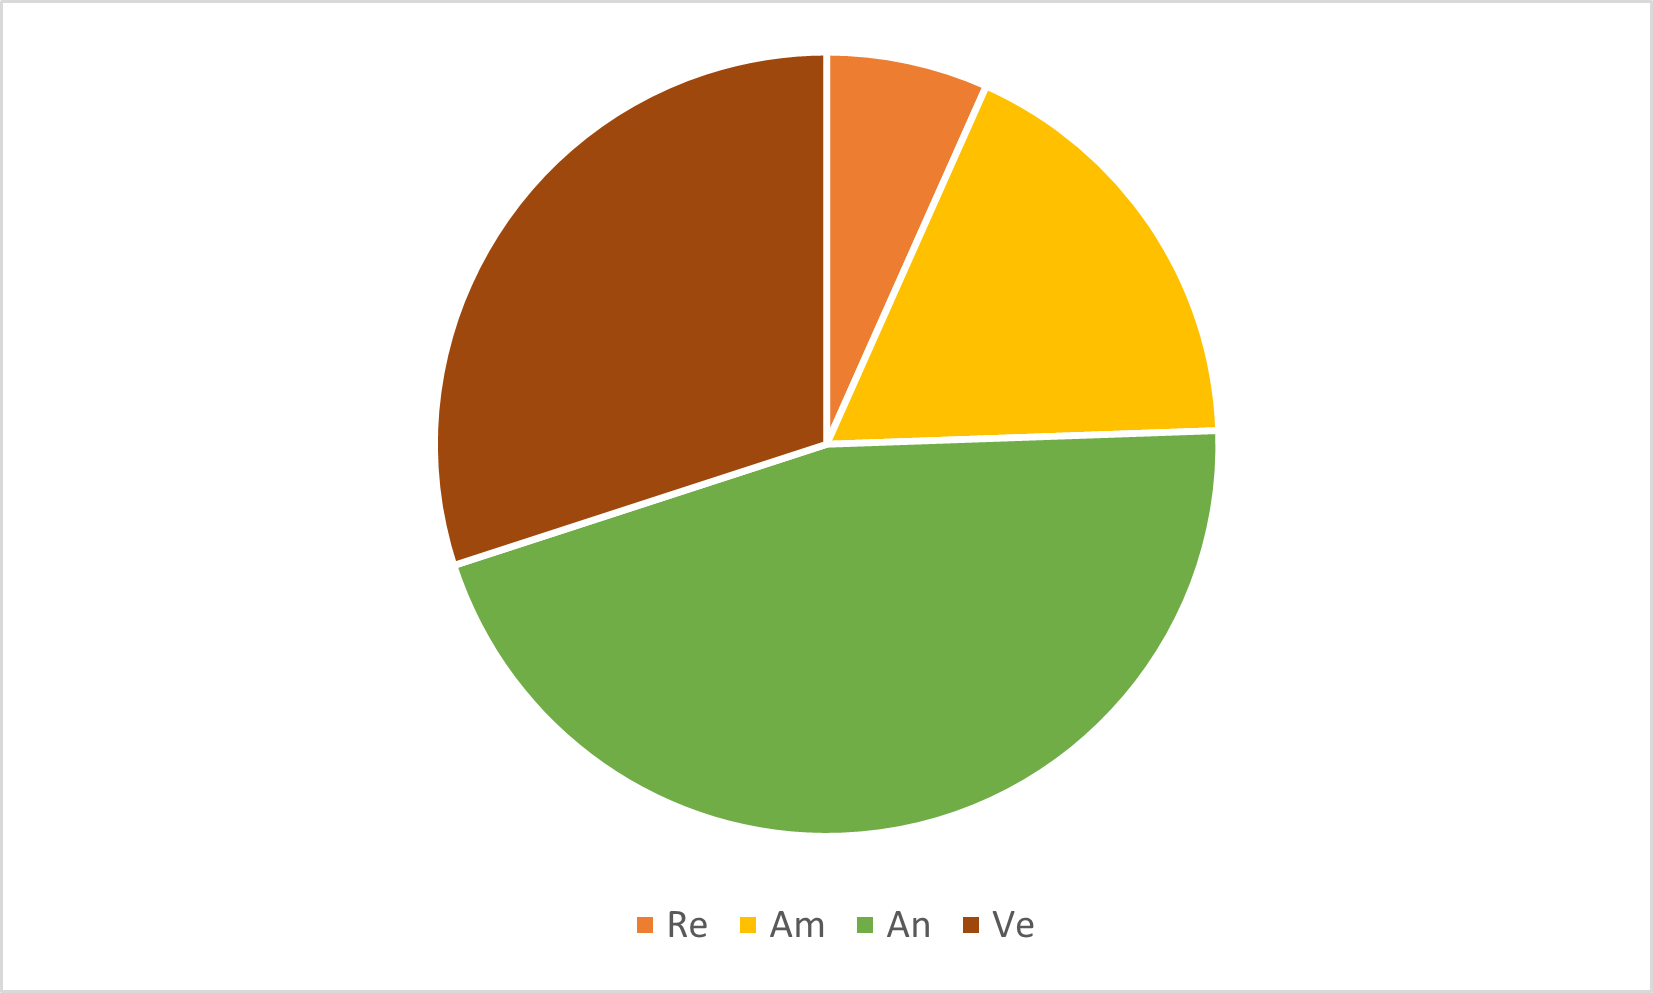
\includegraphics[scale=0.6]{img/grafi preventivo/torta/analisi/sprint2.png}
    \caption{Grafico a torta con la ripartizione delle ore per ruolo nel secondo sprint\textsubscript{G}}
\end{figure}
\subsubsubsection{Preventivo dei costi}
La seguente tabella rappresenta le ore dedicate ad ogni ruolo e il corrispettivo costo in euro per il secondo sprint\textsubscript{G}, svolto nel periodo di analisi:

	\setlength\extrarowheight{5pt}
	\rowcolors{2}{gray!10}{gray!40}
	\begin{tabularx}{\textwidth}{|ccc|c|}
		\hline
		\rowcolor{white}
		\textbf{Ruolo} & \textbf{Costo orario (€)} & \textbf{Ore totali} & \textbf{Costo totale (€)} \\
		\hline
		Responsabile &30&6&180 \\
		Amministratore &20&16&320 \\
		Analista &25&41&1025 \\
		Verificatore &15&27&405 \\
		Programmatore &15&0&0 \\
		Progettista &25&0&0 \\
		\hline
		Totale &-&-&1930 \\
		\hline
		\rowcolor{white}
		\caption{Prospetto del costo orario durante il secondo sprint\textsubscript{G} per ruolo}
	\end{tabularx}
    \vspace{10pt}
	
%
% ----------------------------------------------------------------------------------------------------------------
\newpage
\subsubsection{Sprint\textsubscript{G} III}
% ----------------------------------------------------------------------------------------------------------------
%
\subsubsubsection{Preventivo orario}
La seguente tabella rappresenta la distribuzione oraria di ogni membro del gruppo per il terzo sprint\textsubscript{G} del progetto, il quale è svolto nel periodo di analisi:

	\setlength\extrarowheight{5pt}
	\rowcolors{2}{gray!10}{gray!40}
	\begin{tabularx}{\textwidth}{|ccccccc|c|}
		\hline
		\rowcolor{white}
		\textbf{Nome} & \textbf{Re} & \textbf{Am} & \textbf{An} & \textbf{Ve} & \textbf{Pr}& \textbf{Pt} & \textbf{Ore totali} \\
		\hline
		Nicola Sinicato &0&1&1&3&0&0&5 \\
		Gabriele Da Re &1&2&1&1&0&0&5 \\
		Luca Brugnera &0&2&1&2&0&0&5 \\
		Matteo Stocco &1&1&2&1&0&0&5 \\
		Ana Lazic &1&0&1&3&0&0&5 \\
		Zhen Wei Zheng &0&0&2&3&0&0&5 \\
		\hline
		Ore totali ruolo &3&6&8&13&0&0&30 \\
		\hline
		\rowcolor{white}
		\caption{Distribuzione oraria durante il terzo sprint\textsubscript{G} per ruolo e persona}
	\end{tabularx}
	\vspace{10pt}
	
\begin{figure}[H]
    \centering
    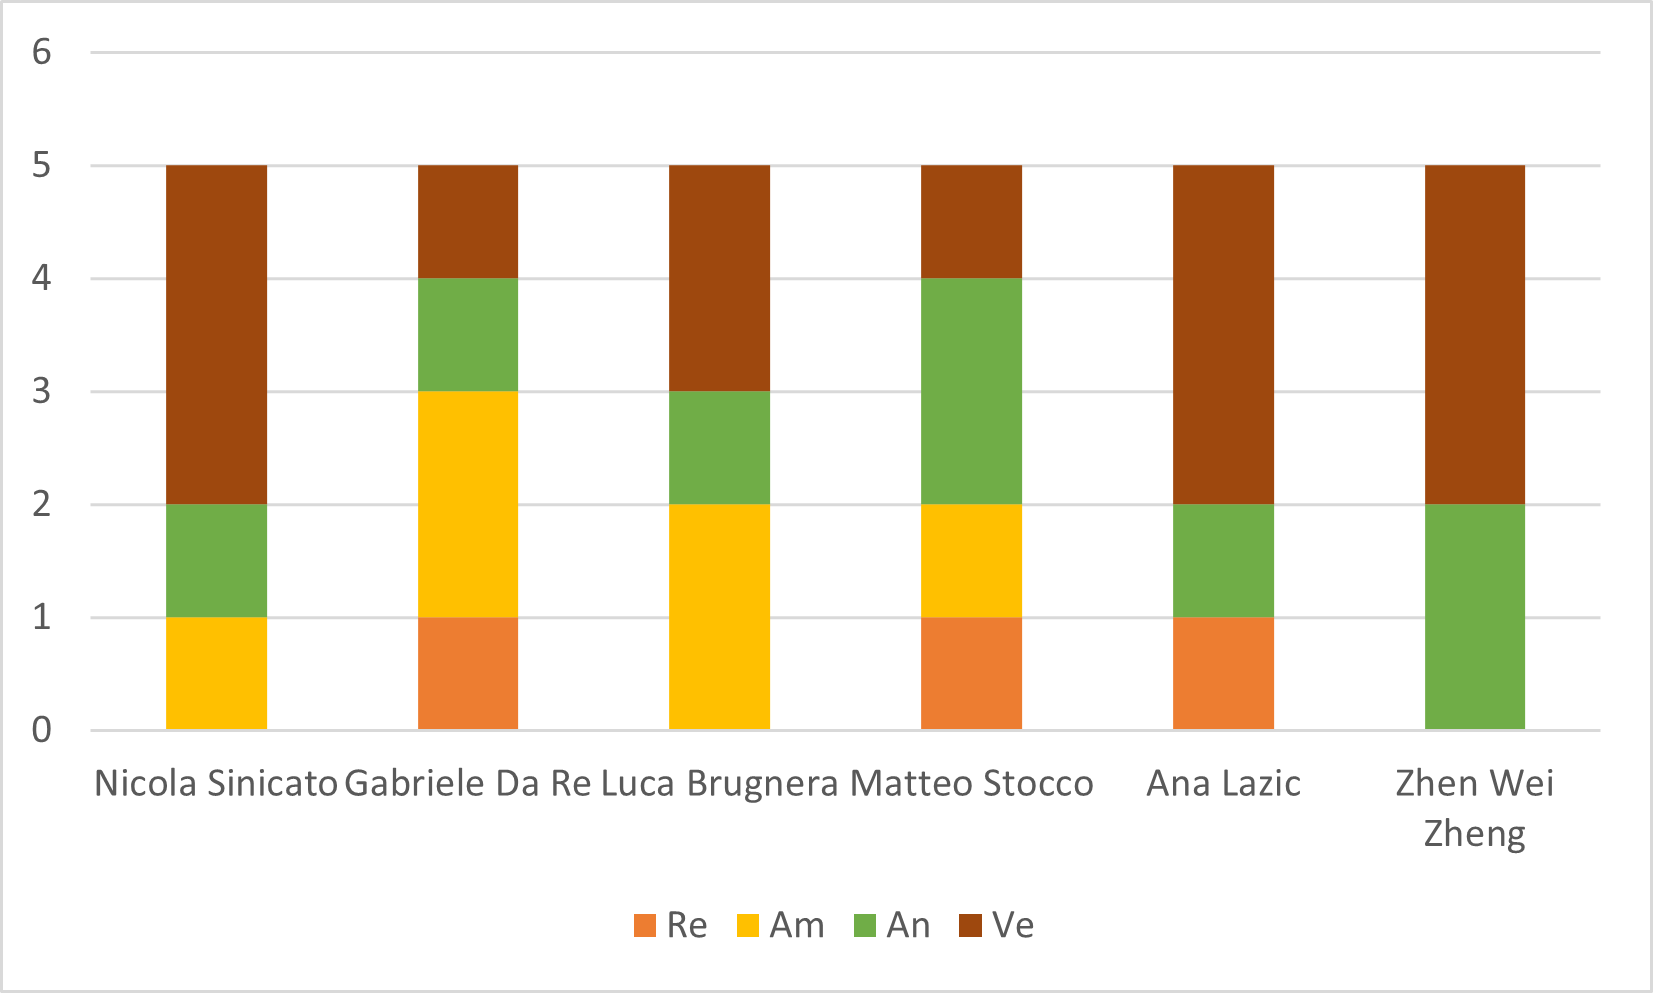
\includegraphics[scale=0.6]{img/grafi preventivo/istogrammi/analisi/sprint3.png}
    \caption{Istogramma con la ripartizione delle ore del primo sprint\textsubscript{G}}
\end{figure}
\begin{figure}[H]
    \centering
    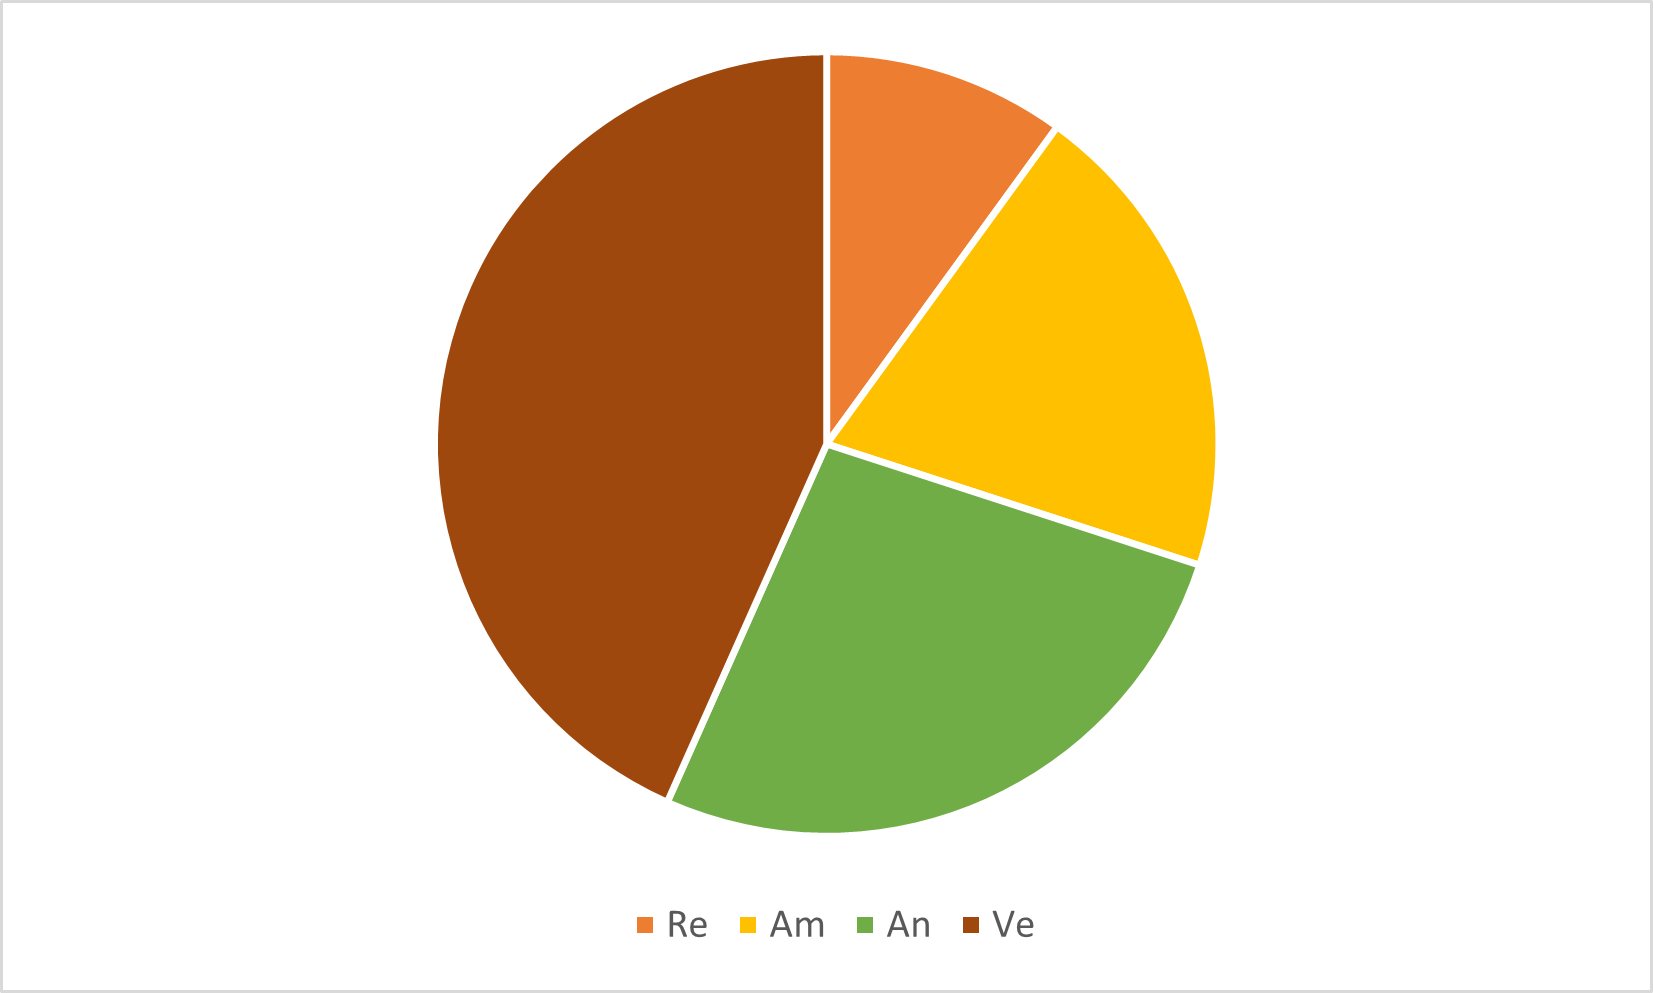
\includegraphics[scale=0.6]{img/grafi preventivo/torta/analisi/sprint3.png}
    \caption{Grafico a torta con la ripartizione delle ore per ruolo nel terzo sprint\textsubscript{G}}
\end{figure}
\subsubsubsection{Preventivo dei costi}
La seguente tabella rappresenta le ore dedicate ad ogni ruolo e il corrispettivo costo in euro per il terzo sprint\textsubscript{G}, svolto nel periodo di analisi:

	\setlength\extrarowheight{5pt}
	\rowcolors{2}{gray!10}{gray!40}
	\begin{tabularx}{\textwidth}{|ccc|c|}
		\hline
		\rowcolor{white}
		\textbf{Ruolo} & \textbf{Costo orario (€)} & \textbf{Ore totali} & \textbf{Costo totale (€)} \\
		\hline
		Responsabile &30&3&90 \\
		Amministratore &20&6&120 \\
		Analista &25&8&200 \\
		Verificatore &15&13&195 \\
		Programmatore &15&0&0 \\
		Progettista &25&0&0 \\
		\hline
		Totale &-&-&605 \\
		\hline
		\rowcolor{white}
		\caption{Prospetto del costo orario durante il terzo sprint\textsubscript{G} per ruolo}
	\end{tabularx}
    \vspace{10pt}
\newpage
\subsubsection{Sprint\textsubscript{G} V}
% ----------------------------------------------------------------------------------------------------------------
%
\subsubsubsection{Preventivo orario}
La seguente tabella rappresenta la distribuzione oraria di ogni membro del gruppo per il quinto sprint\textsubscript{G} del progetto, il quale è svolto nel periodo di analisi in parallelo con il periodo di produzione del proof of concept:

\setlength\extrarowheight{5pt}
\rowcolors{2}{gray!10}{gray!40}
\begin{tabularx}{\textwidth}{|ccccccc|c|}
	\hline
	\rowcolor{white}
	\textbf{Nome} & \textbf{Re} & \textbf{Am} & \textbf{An} & \textbf{Ve} & \textbf{Pr}& \textbf{Pt} & \textbf{Ore totali} \\
	\hline
	Nicola Sinicato &0&1&1&1&0&0&3 \\
	Gabriele Da Re &1&1&0&1&0&0&3 \\
	Luca Brugnera &0&0&2&1&0&0&3 \\
	Matteo Stocco &1&1&0&1&0&0&3 \\
	Ana Lazic &0&0&2&1&0&0&3 \\
	Zhen Wei Zheng &1&0&0&2&0&0&3 \\
	\hline
	Ore totali ruolo &3&3&5&7&0&0&18 \\
	\hline
	\rowcolor{white}
	\caption{Distribuzione oraria durante il quinto sprint\textsubscript{G} per ruolo e persona}
\end{tabularx}
\vspace{10pt}

\begin{figure}[H]
	\centering
	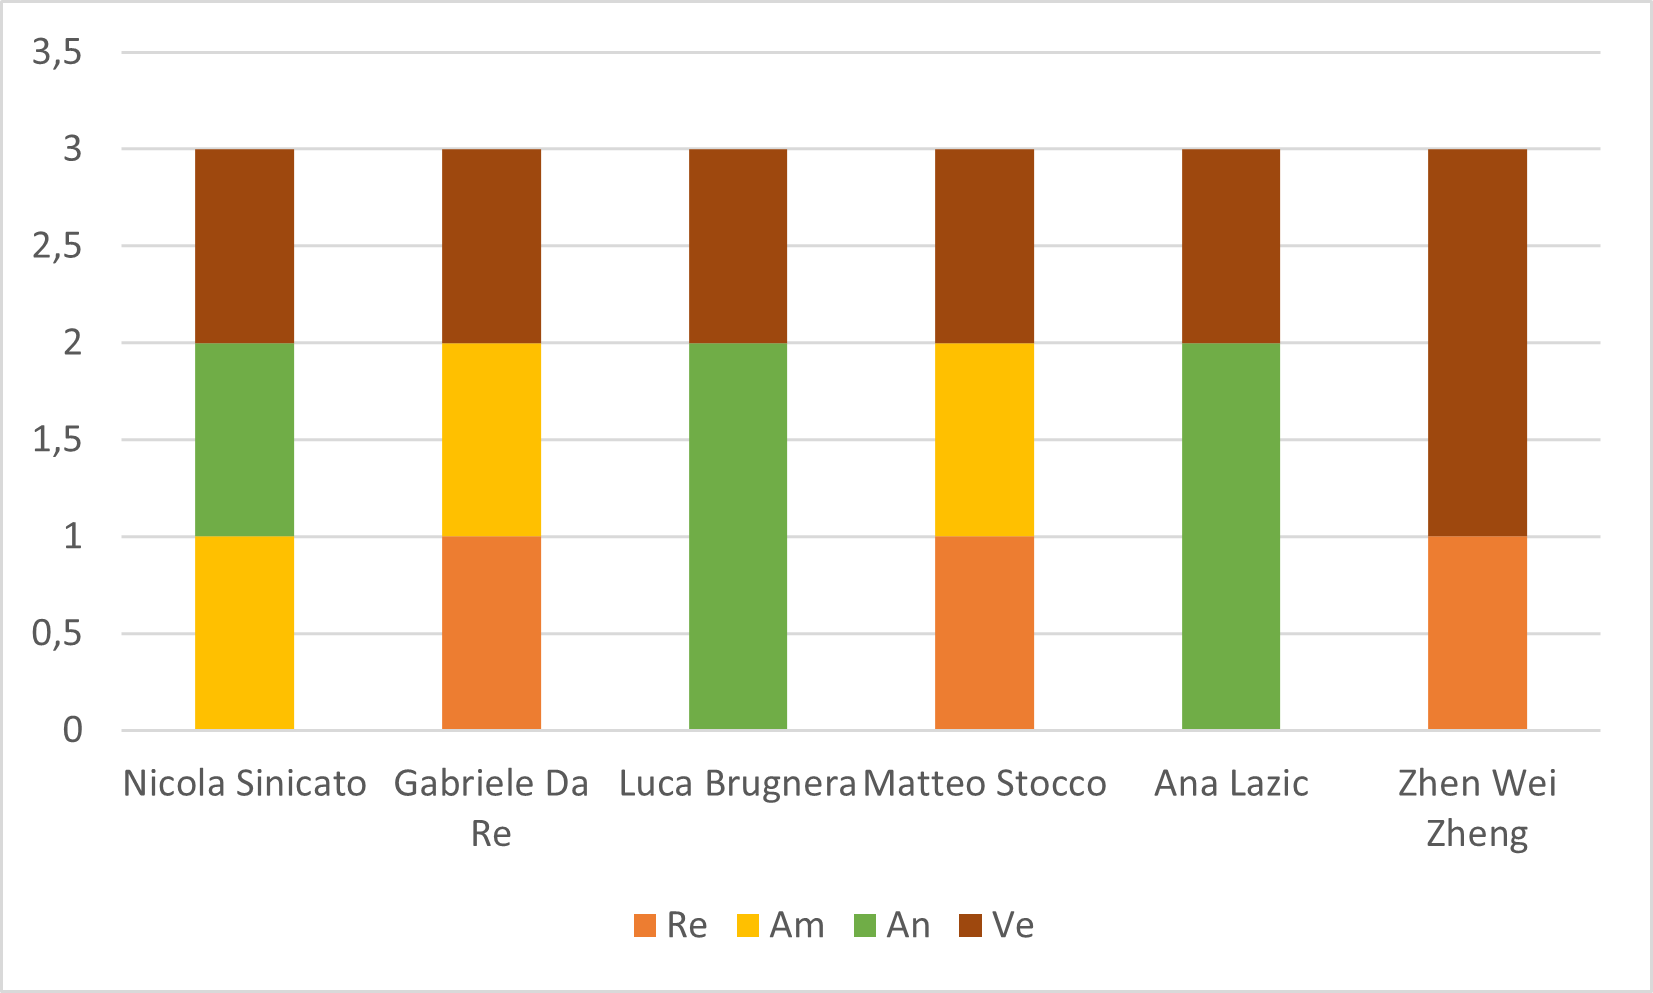
\includegraphics[scale=0.6]{img/grafi preventivo/istogrammi/analisi/sprint5.png}
	\caption{Istogramma con la ripartizione delle ore del quinto sprint\textsubscript{G}}
\end{figure}
\begin{figure}[H]
	\centering
	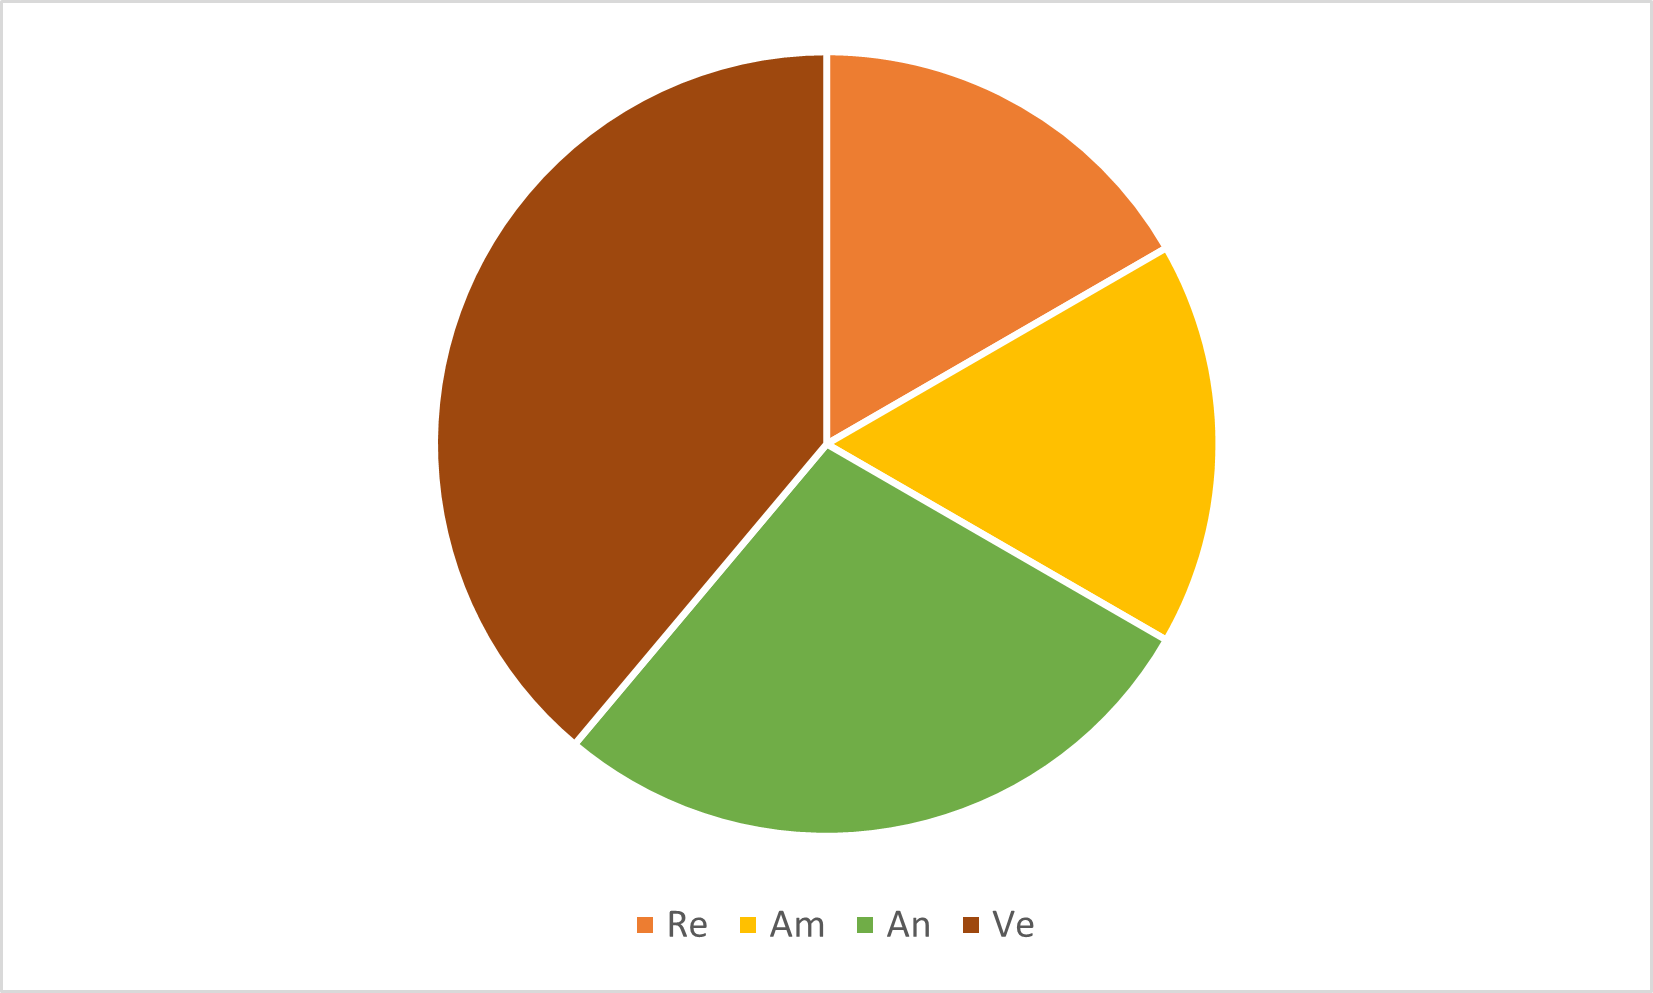
\includegraphics[scale=0.6]{img/grafi preventivo/torta/analisi/sprint5.png}
	\caption{Grafico a torta con la ripartizione delle ore per ruolo nel quinto sprint\textsubscript{G}}
\end{figure}
\subsubsubsection{Preventivo dei costi}
La seguente tabella rappresenta le ore dedicate ad ogni ruolo e il corrispettivo costo in euro per il quinto sprint\textsubscript{G}, svolto nel periodo di analisi in parallelo con il periodo di produzione del proof of concept:

\setlength\extrarowheight{5pt}
\rowcolors{2}{gray!10}{gray!40}
\begin{tabularx}{\textwidth}{|ccc|c|}
	\hline
	\rowcolor{white}
	\textbf{Ruolo} & \textbf{Costo orario (€)} & \textbf{Ore totali} & \textbf{Costo totale (€)} \\
	\hline
	Responsabile &30&3&90 \\
	Amministratore &20&3&60 \\
	Analista &25&5&125 \\
	Verificatore &15&7&105 \\
	Programmatore &15&0&0 \\
	Progettista &25&0&0 \\
	\hline
	Totale &-&-&380 \\
	\hline
	\rowcolor{white}
	\caption{Prospetto del costo orario durante il quinto sprint\textsubscript{G} per ruolo}
\end{tabularx}
\vspace{10pt}
%
% ----------------------------------------------------------------------------------------------------------------
\newpage
\subsubsection{Sprint\textsubscript{G} VI}
% ----------------------------------------------------------------------------------------------------------------
%
\subsubsubsection{Preventivo orario}
La seguente tabella rappresenta la distribuzione oraria di ogni membro del gruppo per il sesto sprint\textsubscript{G} del progetto, il quale è svolto nel periodo di validazione\textsubscript{G} e collaudo:

\setlength\extrarowheight{5pt}
\rowcolors{2}{gray!10}{gray!40}
\begin{tabularx}{\textwidth}{|ccccccc|c|}
	\hline
	\rowcolor{white}
	\textbf{Nome} & \textbf{Re} & \textbf{Am} & \textbf{An} & \textbf{Ve} & \textbf{Pr}& \textbf{Pt} & \textbf{Ore totali} \\
	\hline
	Nicola Sinicato &0&0&0&3&0&0&3 \\
	Gabriele Da Re &1&0&0&2&0&0&3\\
	Luca Brugnera &0&1&0&2&0&0&3 \\
	Matteo Stocco &1&1&0&2&0&0&4 \\
	Ana Lazic &0&1&0&3&0&0&4 \\
	Zhen Wei Zheng &0&1&0&2&0&0&3 \\
	\hline
	Ore totali ruolo &2&4&0&14&0&0&20 \\
	\hline
	\rowcolor{white}
	\caption{Distribuzione oraria durante il sesto sprint\textsubscript{G} per ruolo e persona}
\end{tabularx}
\vspace{10pt}

\begin{figure}[H]
	\centering
	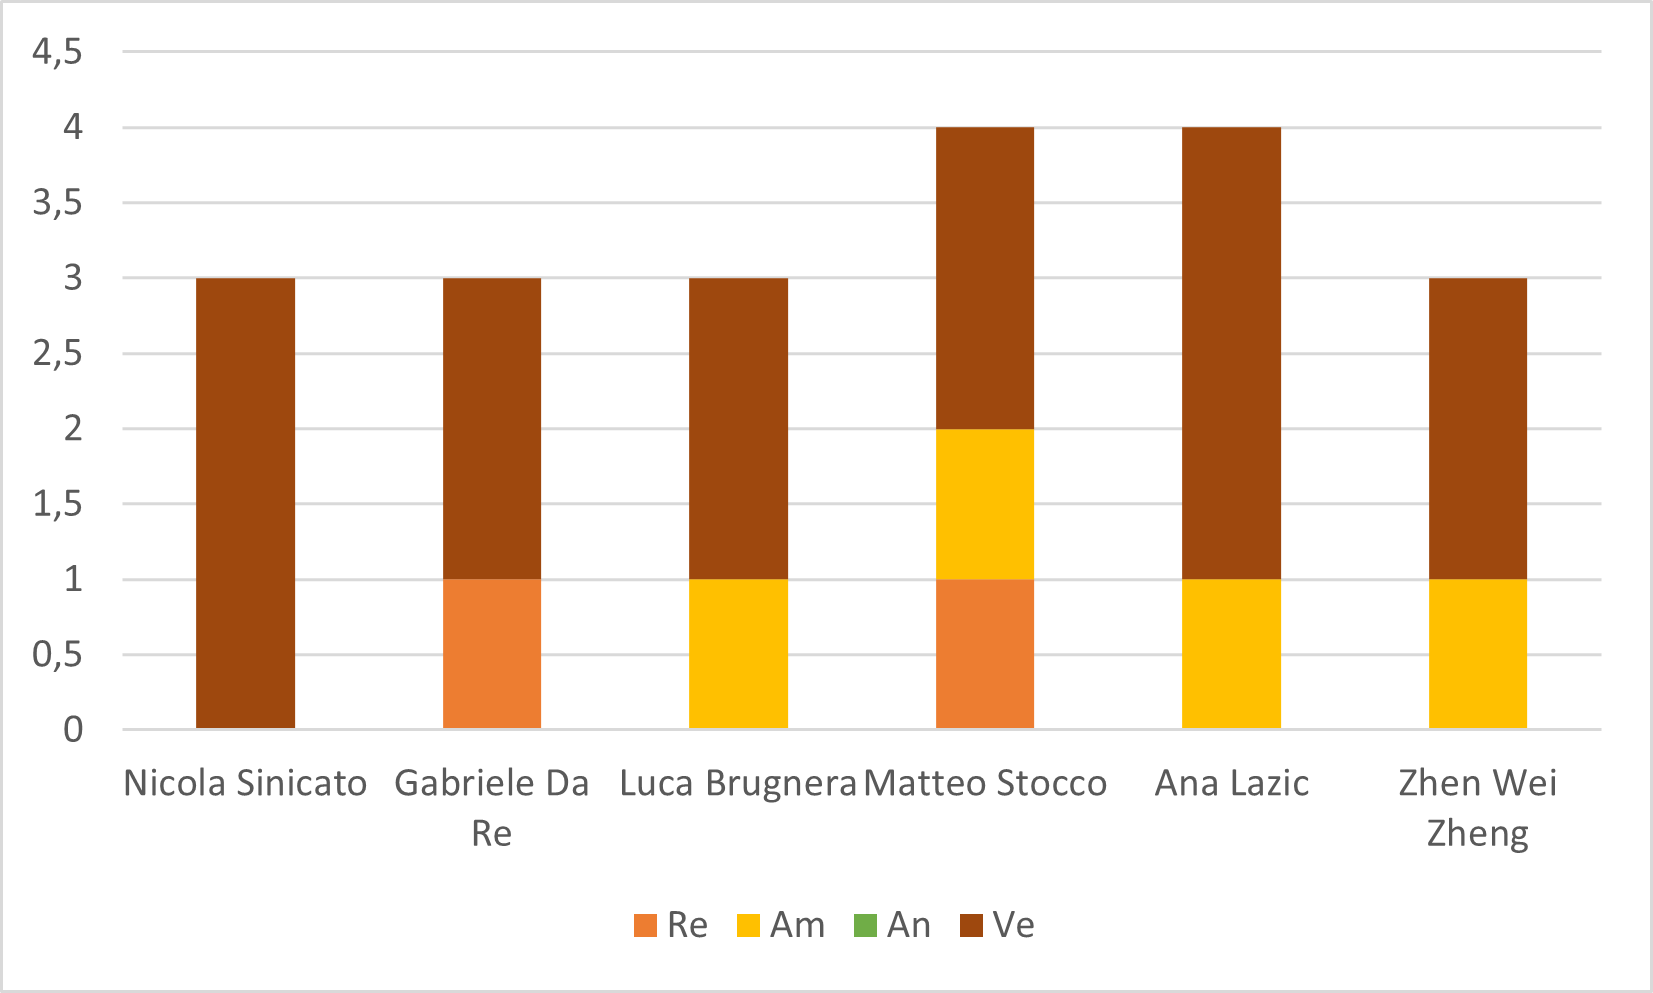
\includegraphics[scale=0.6]{img/grafi preventivo/istogrammi/analisi/sprint6.png}
	\caption{Istogramma con la ripartizione delle ore del sesto sprint\textsubscript{G}}
\end{figure}
\begin{figure}[H]
	\centering
	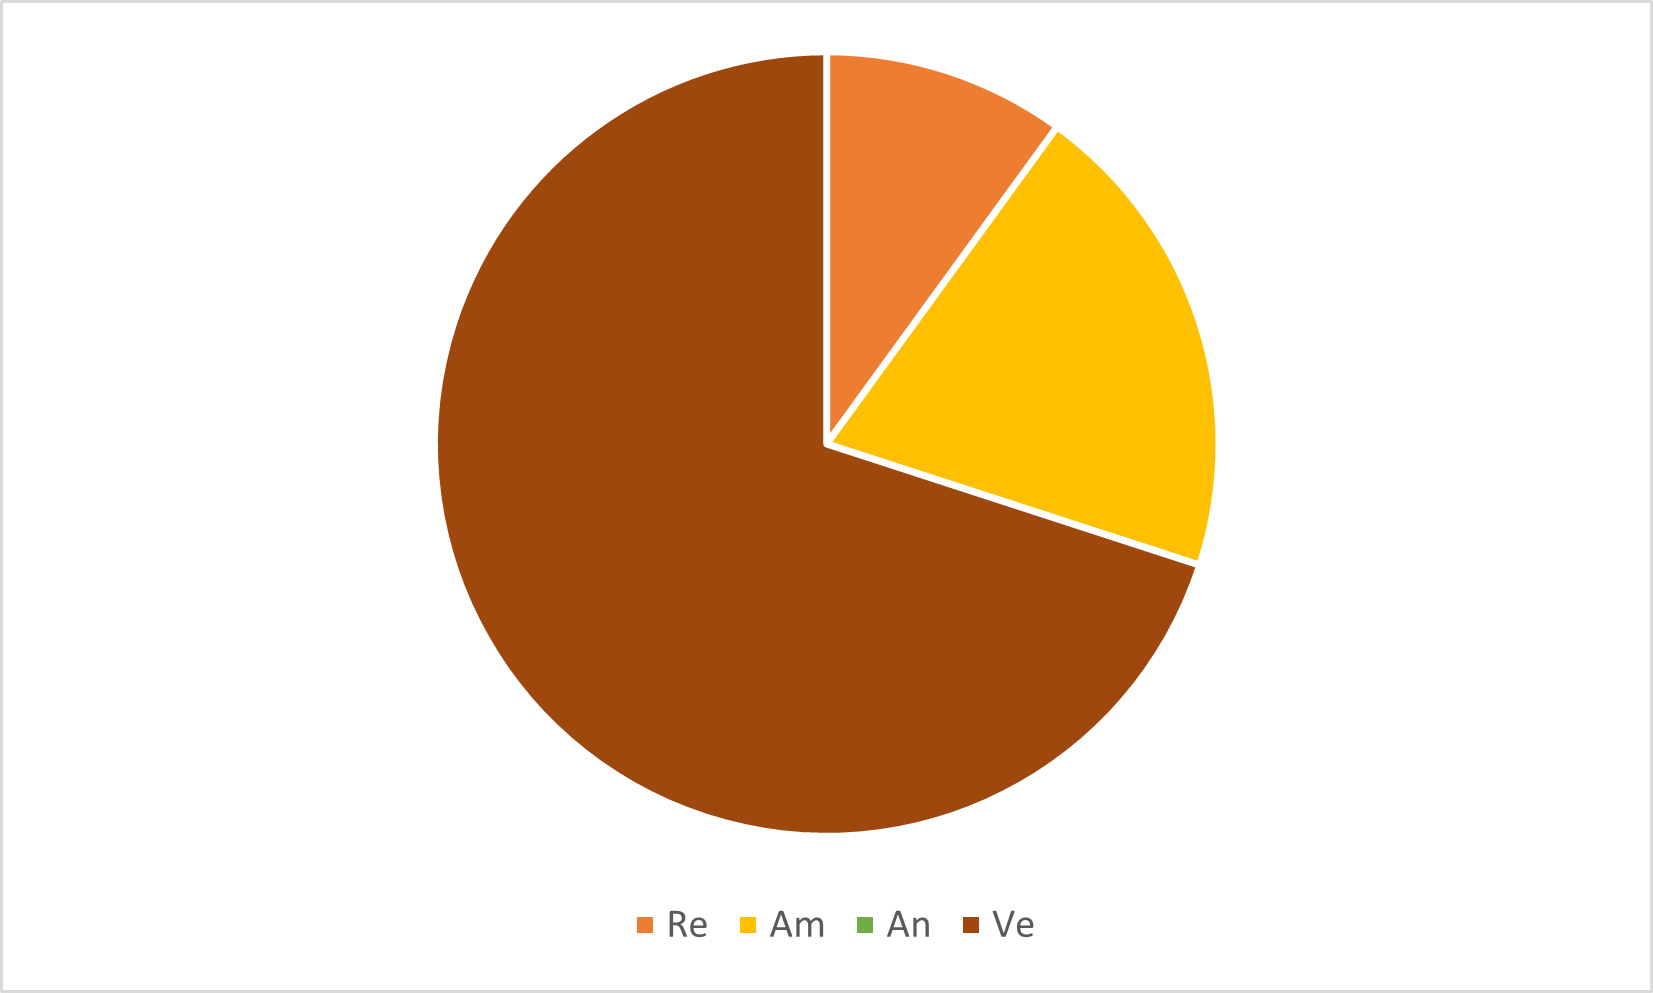
\includegraphics[scale=0.6]{img/grafi preventivo/torta/analisi/sprint6.png}
	\caption{Grafico a torta con la ripartizione delle ore per ruolo nel sesto sprint\textsubscript{G}}
\end{figure}
\subsubsubsection{Preventivo dei costi}
La seguente tabella rappresenta le ore dedicate ad ogni ruolo e il corrispettivo costo in euro per il sesto sprint\textsubscript{G}, svolto nel periodo di validazione\textsubscript{G} e collaudo:

\setlength\extrarowheight{5pt}
\rowcolors{2}{gray!10}{gray!40}
\begin{tabularx}{\textwidth}{|ccc|c|}
	\hline
	\rowcolor{white}
	\textbf{Ruolo} & \textbf{Costo orario (€)} & \textbf{Ore totali} & \textbf{Costo totale (€)} \\
	\hline
	Responsabile &30&2&60 \\
	Amministratore &20&4&80 \\
	Analista &25&0&0 \\
	Verificatore &15&14&210 \\
	Programmatore &15&0&0 \\
	Progettista &25&0&0 \\
	\hline
	Totale &-&-&350 \\
	\hline
	\rowcolor{white}
	\caption{Prospetto del costo orario durante il sesto sprint\textsubscript{G} per ruolo}
\end{tabularx}
\vspace{10pt}

% ----------------------------------------------------------------------------------------------------------------
\newpage
\subsubsection{Riepilogo del periodo di analisi}
% ----------------------------------------------------------------------------------------------------------------
%
\subsubsubsection{Preventivo orario}
La seguente tabella rappresenta la distribuzione oraria per ogni membro del gruppo per il periodo di analisi:

	\setlength\extrarowheight{5pt}
	\rowcolors{2}{gray!10}{gray!40}
	\begin{tabularx}{\textwidth}{|ccccccc|c|}
		\hline
		\rowcolor{white}
		\textbf{Nome} & \textbf{Re} & \textbf{Am} & \textbf{An} & \textbf{Ve} & \textbf{Pr}& \textbf{Pt} & \textbf{Ore totali} \\
		\hline
		Nicola Sinicato &5&6&14&11&0&0&36 \\
		Gabriele Da Re &4&13&12&7&0&0&36 \\
		Luca Brugnera &1&14&13&8&0&0&36 \\
		Matteo Stocco &6&10&13&8&0&0&37 \\
		Ana Lazic &2&6&16&13&0&0&37 \\
		Zhen Wei Zheng &2&6&14&14&0&0&36 \\
		\hline
		Ore totali ruolo &20&55&82&61&0&0&218 \\
		\hline
		\rowcolor{white}
		\caption{Distribuzione oraria durante il periodo di analisi per ruolo e persona}
	\end{tabularx}
	\vspace{10pt}
	
\begin{figure}[H]
    \centering
    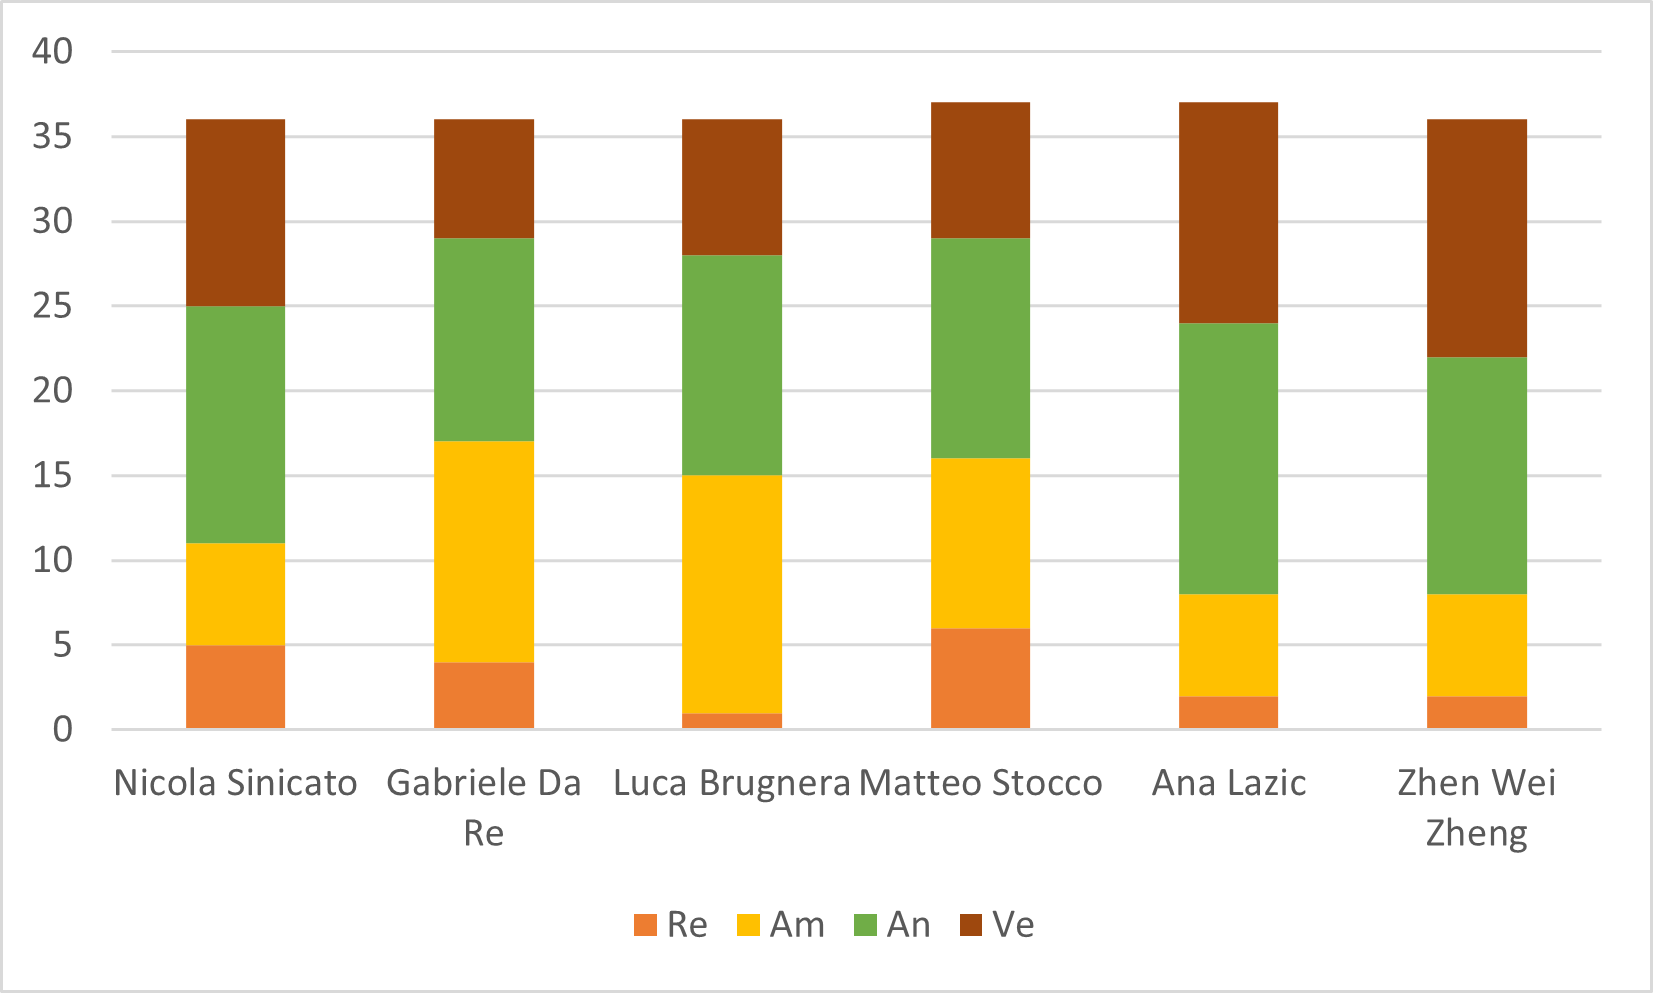
\includegraphics[scale=0.6]{img/grafi preventivo/istogrammi/analisi/complessivo.png}
    \caption{Istogramma con la ripartizione delle ore nel periodo di analisi}
\end{figure}
\begin{figure}[H]
    \centering
    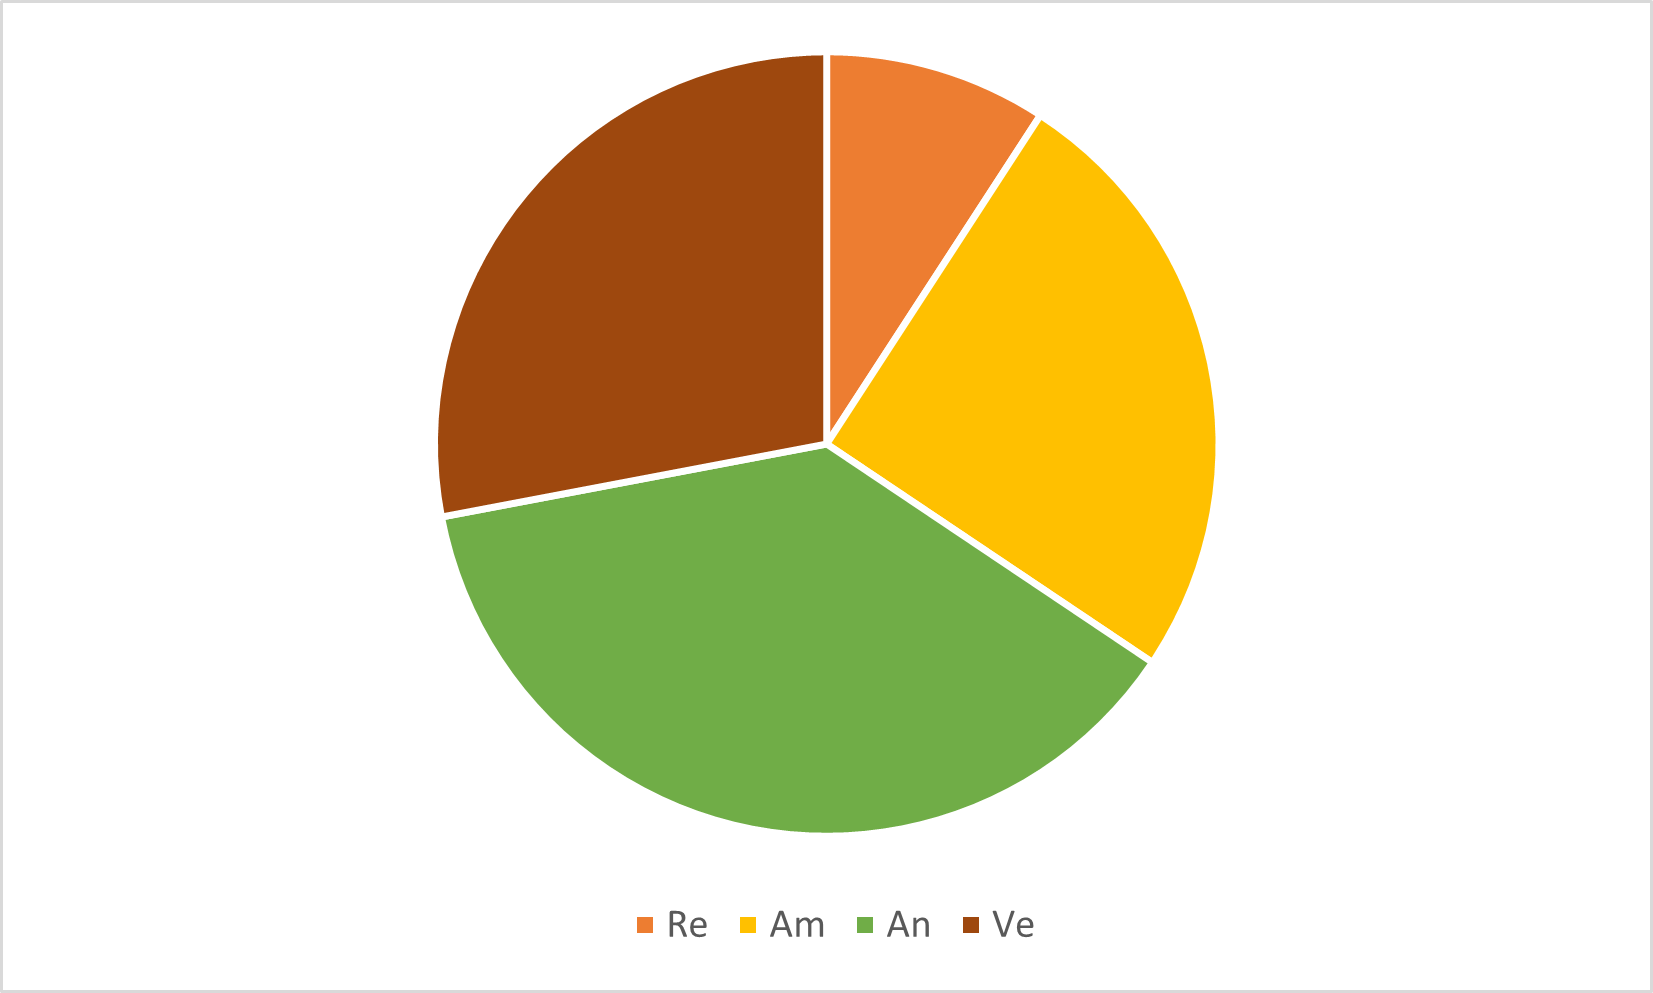
\includegraphics[scale=0.6]{img/grafi preventivo/torta/analisi/complessivo.png}
    \caption{Grafico a torta con la ripartizione delle ore per ruolo nel periodo di analisi}
\end{figure}
\subsubsubsection{Preventivo dei costi}
La seguente tabella rappresenta le ore dedicate ad ogni ruolo e il corrispettivo costo in euro per il periodo di analisi:

	\setlength\extrarowheight{5pt}
	\rowcolors{2}{gray!10}{gray!40}
	\begin{tabularx}{\textwidth}{|ccc|c|}
		\hline
		\rowcolor{white}
		\textbf{Ruolo} & \textbf{Costo orario (€)} & \textbf{Ore totali} & \textbf{Costo totale (€)} \\
		\hline
		Responsabile &30&20&600 \\
		Amministratore &20&55&1100 \\
		Analista &25&82&2050 \\
		Verificatore &15&61&915 \\
		Programmatore &15&0&0 \\
		Progettista &25&0&0 \\
		\hline
		Totale &-&-&4665 \\
		\hline
		\rowcolor{white}
		\caption{Prospetto del costo orario durante il periodo di analisi per ruolo}
	\end{tabularx}
    \vspace{10pt}
	
% ----------------------------------------------------------------------------------------------------------------
%
\newpage
\subsection{Produzione del proof of concept}

% ----------------------------------------------------------------------------------------------------------------
\subsubsection{Sprint\textsubscript{G} IV}
% ----------------------------------------------------------------------------------------------------------------
%
\subsubsubsection{Preventivo orario}
La seguente tabella rappresenta la distribuzione oraria di ogni membro del gruppo per il quarto sprint\textsubscript{G} del progetto, il quale è svolto nel periodo di produzione del proof of concept:

	\setlength\extrarowheight{5pt}
	\rowcolors{2}{gray!10}{gray!40}
	\begin{tabularx}{\textwidth}{|ccccccc|c|}
		\hline
		\rowcolor{white}
		\textbf{Nome} & \textbf{Re} & \textbf{Am} & \textbf{An} & \textbf{Ve} & \textbf{Pr}& \textbf{Pt} & \textbf{Ore totali} \\
		\hline
		Nicola Sinicato &1&0&0&0&1&1&3 \\
		Gabriele Da Re &0&1&0&0&0&2&3 \\
		Luca Brugnera &1&0&0&1&0&1&3 \\
		Matteo Stocco &0&0&1&1&0&1&3 \\
		Ana Lazic &1&0&0&0&1&1&3 \\
		Zhen Wei Zheng &0&1&1&0&0&1&3 \\
		\hline
		Ore totali ruolo &3&2&2&2&2&7&18 \\
		\hline
		\rowcolor{white}
		\caption{Distribuzione oraria durante il quarto sprint\textsubscript{G} per ruolo e persona}
	\end{tabularx}
	\vspace{10pt}
	
\begin{figure}[H]
    \centering
    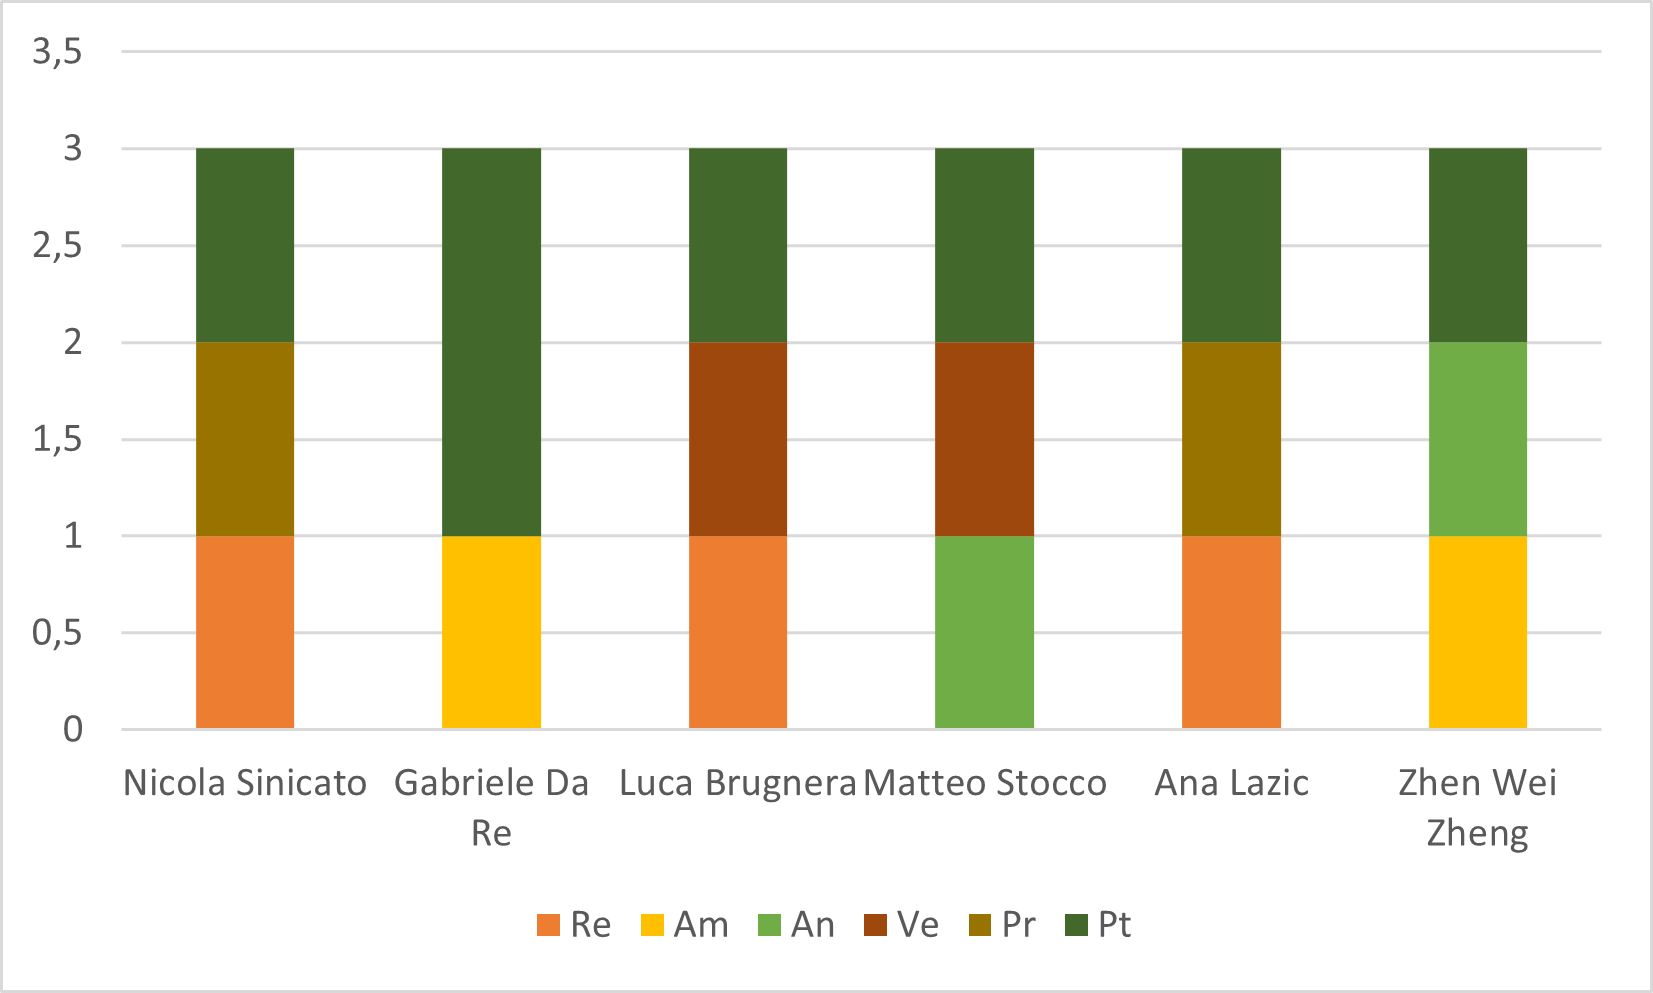
\includegraphics[scale=0.6]{img/grafi preventivo/istogrammi/proof/sprint4.png}
    \caption{Istogramma con la ripartizione delle ore del quarto sprint\textsubscript{G}}
\end{figure}
\begin{figure}[H]
    \centering
    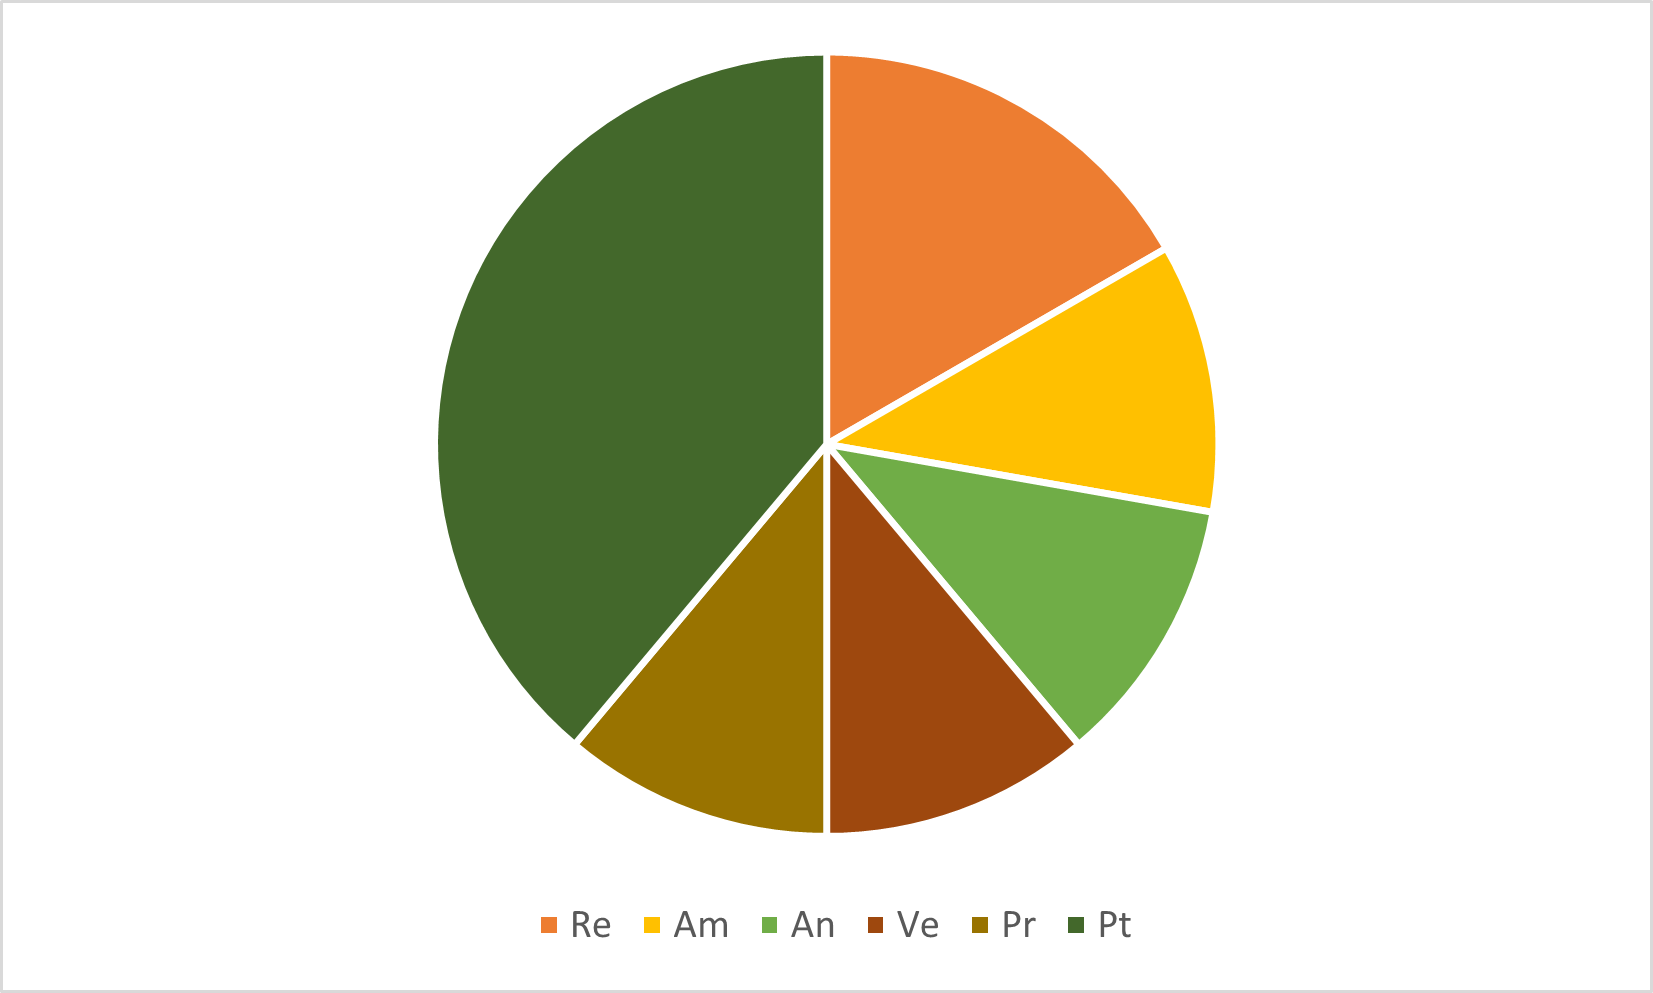
\includegraphics[scale=0.6]{img/grafi preventivo/torta/proof/sprint4.png}
    \caption{Grafico a torta con la ripartizione delle ore per ruolo nel quarto sprint\textsubscript{G}}
\end{figure}
\subsubsubsection{Preventivo dei costi}
La seguente tabella rappresenta le ore dedicate ad ogni ruolo e il corrispettivo costo in euro per il quarto sprint\textsubscript{G}, svolto nel periodo di produzione del proof of concept:

	\setlength\extrarowheight{5pt}
	\rowcolors{2}{gray!10}{gray!40}
	\begin{tabularx}{\textwidth}{|ccc|c|}
		\hline
		\rowcolor{white}
		\textbf{Ruolo} & \textbf{Costo orario (€)} & \textbf{Ore totali} & \textbf{Costo totale (€)} \\
		\hline
		Responsabile &30&3&90 \\
		Amministratore &20&2&40 \\
		Analista &25&2&50 \\
		Verificatore &15&2&30 \\
		Programmatore &15&2&30 \\
		Progettista &25&7&175 \\
		\hline
		Totale &-&-&415 \\
		\hline
		\rowcolor{white}
		\caption{Prospetto del costo orario durante il quarto sprint\textsubscript{G} per ruolo}
	\end{tabularx}
    \vspace{10pt}
	
% ----------------------------------------------------------------------------------------------------------------
\newpage
\subsubsection{Sprint\textsubscript{G} V}
% ----------------------------------------------------------------------------------------------------------------
%
\subsubsubsection{Preventivo orario}
La seguente tabella rappresenta la distribuzione oraria di ogni membro del gruppo per il quinto sprint\textsubscript{G} del progetto, il quale è svolto nel periodo di proof of concept in parallelo con il periodo di analisi:

	\setlength\extrarowheight{5pt}
	\rowcolors{2}{gray!10}{gray!40}
	\begin{tabularx}{\textwidth}{|ccccccc|c|}
		\hline
		\rowcolor{white}
		\textbf{Nome} & \textbf{Re} & \textbf{Am} & \textbf{An} & \textbf{Ve} & \textbf{Pr}& \textbf{Pt} & \textbf{Ore totali} \\
		\hline
		Nicola Sinicato &0&1&0&1&4&0&6 \\
		Gabriele Da Re &2&0&0&0&1&3&6 \\
		Luca Brugnera &0&0&2&1&3&0&6 \\
		Matteo Stocco &0&1&0&3&2&0&6 \\
		Ana Lazic &0&1&0&0&3&2&6 \\
		Zhen Wei Zheng &1&0&0&2&0&3&6 \\
		\hline
		Ore totali ruolo &3&3&2&7&13&8&36 \\
		\hline
		\rowcolor{white}
		\caption{Distribuzione oraria durante il quinto sprint\textsubscript{G} per ruolo e persona}
	\end{tabularx}
	\vspace{10pt}
	
\begin{figure}[H]
    \centering
    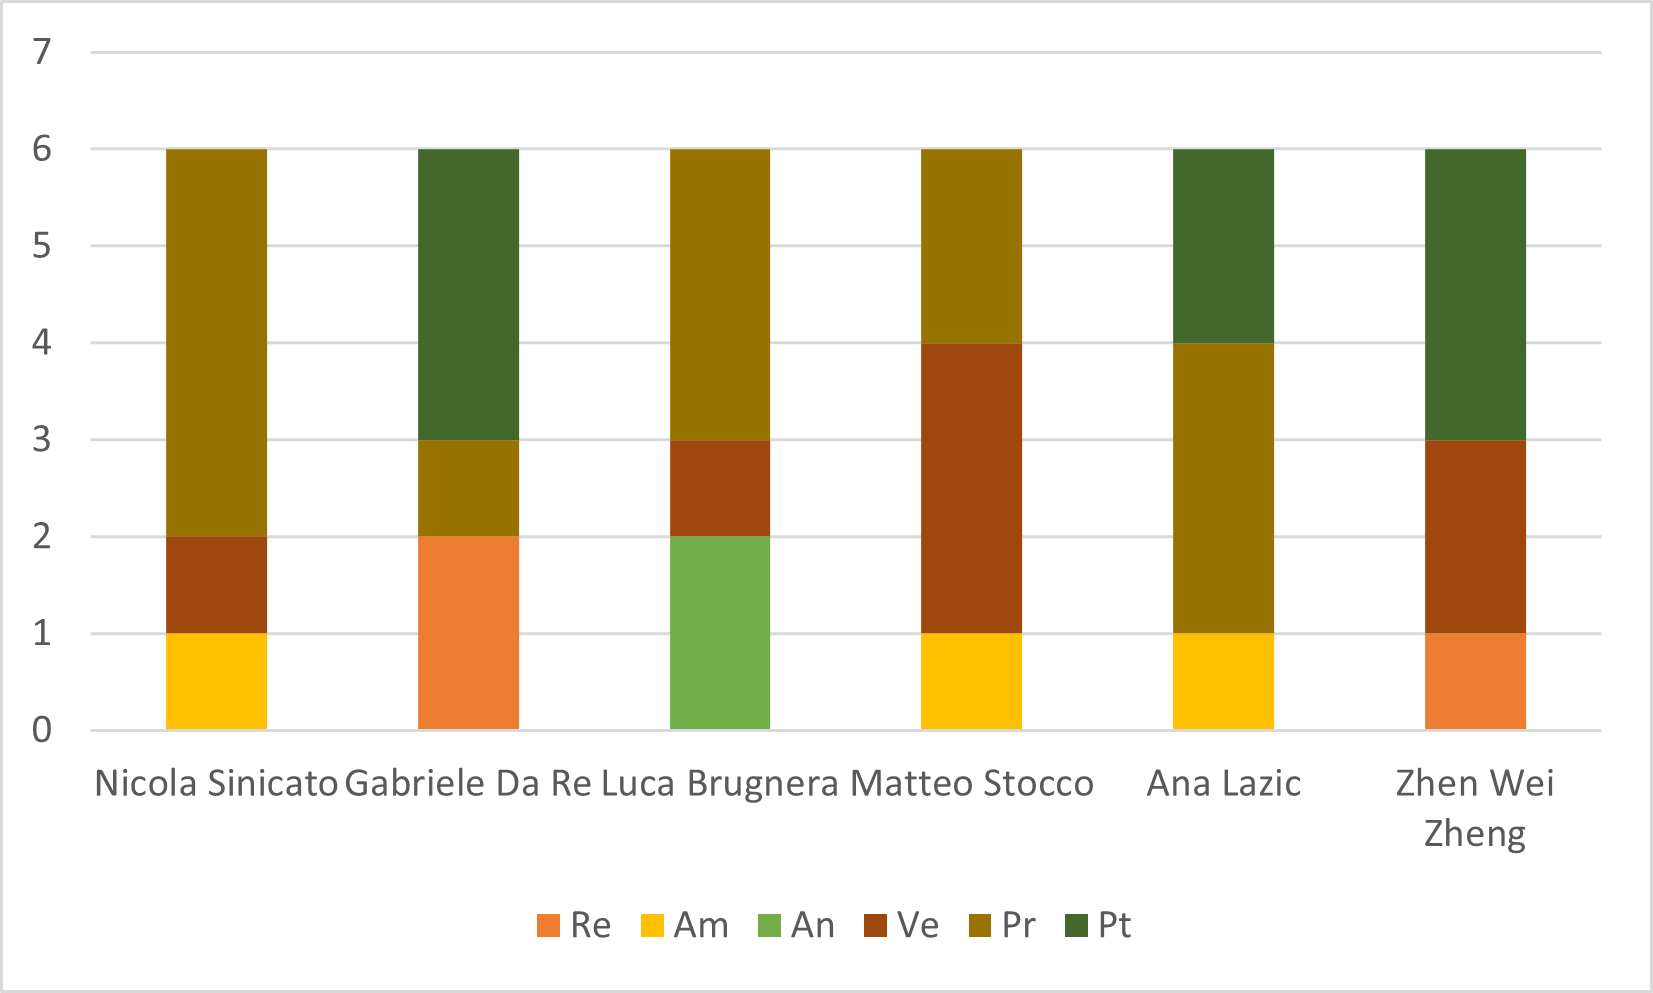
\includegraphics[scale=0.6]{img/grafi preventivo/istogrammi/proof/sprint5.png}
    \caption{Istogramma con la ripartizione delle ore del quinto sprint\textsubscript{G}}
\end{figure}
\begin{figure}[H]
    \centering
    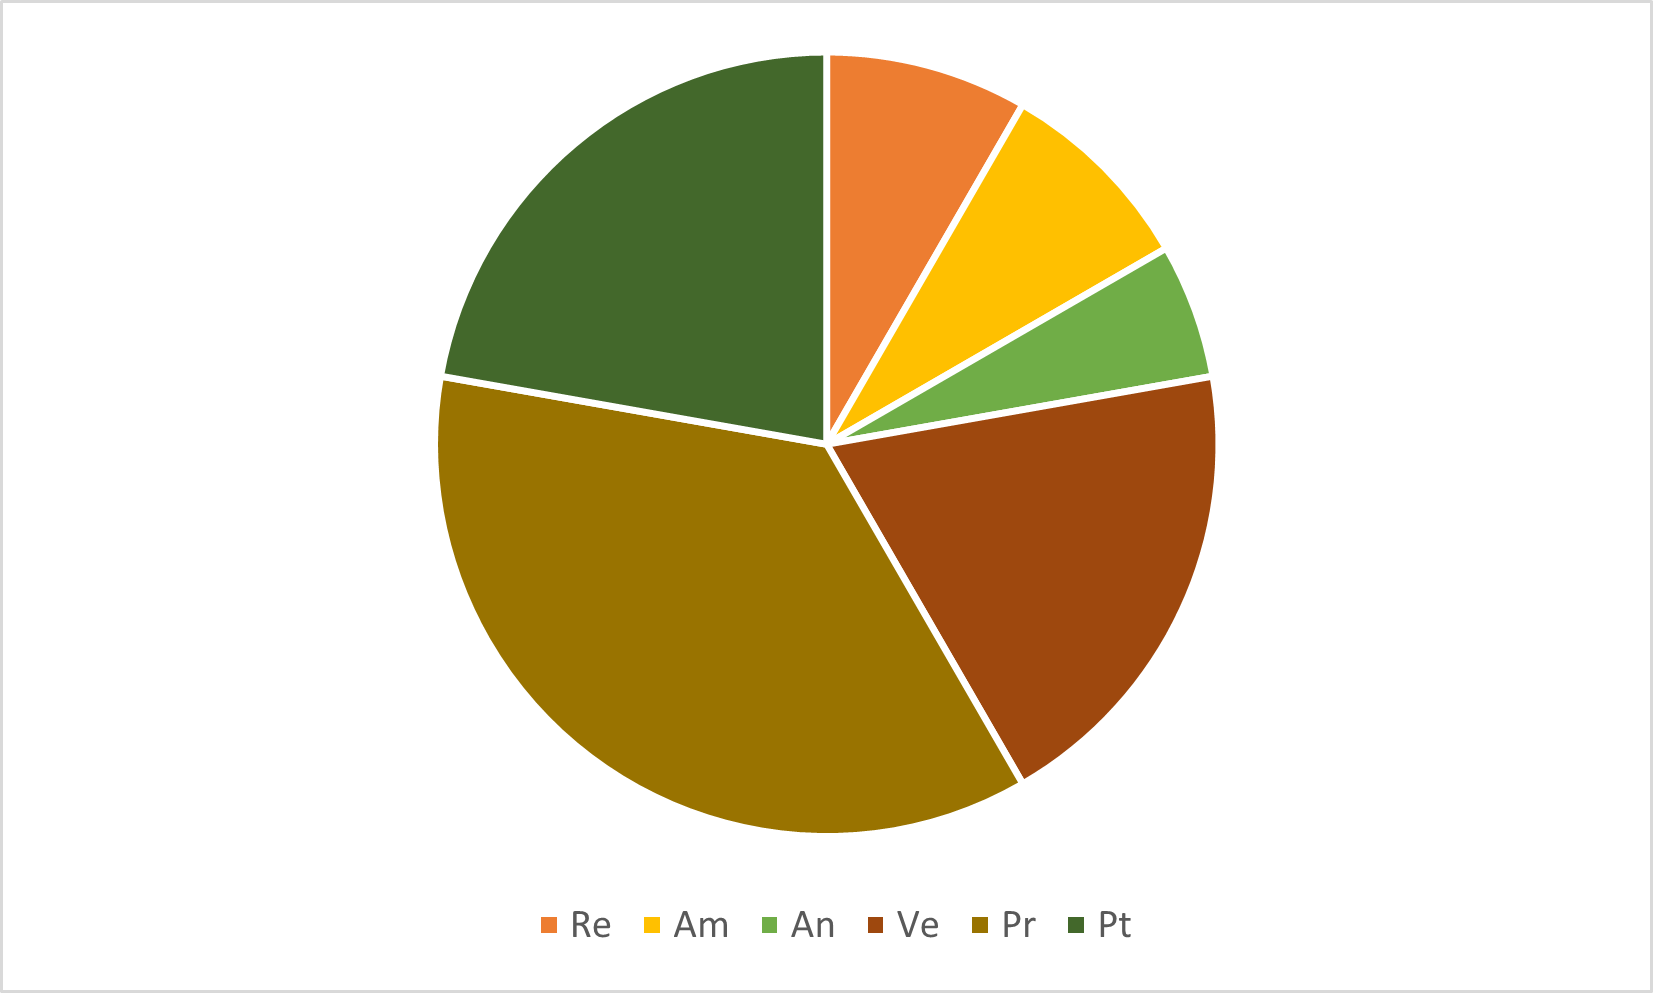
\includegraphics[scale=0.6]{img/grafi preventivo/torta/proof/sprint5.png}
    \caption{Grafico a torta con la ripartizione delle ore per ruolo nel quinto sprint\textsubscript{G}}
\end{figure}
\subsubsubsection{Preventivo dei costi}
La seguente tabella rappresenta le ore dedicate ad ogni ruolo e il corrispettivo costo in euro per il quinto sprint\textsubscript{G}, svolto nel periodo di produzione del proof of concept in parallelo con il periodo di analisi:

	\setlength\extrarowheight{5pt}
	\rowcolors{2}{gray!10}{gray!40}
	\begin{tabularx}{\textwidth}{|ccc|c|}
		\hline
		\rowcolor{white}
		\textbf{Ruolo} & \textbf{Costo orario (€)} & \textbf{Ore totali} & \textbf{Costo totale (€)} \\
		\hline
		Responsabile &30&3&90 \\
		Amministratore &20&3&60 \\
		Analista &25&2&50 \\
		Verificatore &15&7&105 \\
		Programmatore &15&13&195 \\
		Progettista &25&8&200 \\
		\hline
		Totale &-&-&700 \\
		\hline
		\rowcolor{white}
		\caption{Prospetto del costo orario durante il quinto sprint\textsubscript{G} per ruolo}
	\end{tabularx}
    \vspace{10pt}
	
% ----------------------------------------------------------------------------------------------------------------
\newpage
\subsubsection{Riepilogo del periodo di produzione del proof of concept}
% ----------------------------------------------------------------------------------------------------------------
%
\subsubsubsection{Preventivo orario}
La seguente tabella rappresenta la distribuzione oraria per ogni membro del gruppo per il periodo di produzione del proof of concept:

	\setlength\extrarowheight{5pt}
	\rowcolors{2}{gray!10}{gray!40}
	\begin{tabularx}{\textwidth}{|ccccccc|c|}
		\hline
		\rowcolor{white}
		\textbf{Nome} & \textbf{Re} & \textbf{Am} & \textbf{An} & \textbf{Ve} & \textbf{Pr}& \textbf{Pt} & \textbf{Ore totali} \\
		\hline
		Nicola Sinicato &1&1&0&1&5&1&9 \\
		Gabriele Da Re &2&1&0&0&1&5&9 \\
		Luca Brugnera &1&0&2&2&3&1&9 \\
		Matteo Stocco &0&1&1&4&2&1&9 \\
		Ana Lazic &1&1&0&0&4&3&9 \\
		Zhen Wei Zheng &1&1&1&2&0&4&9 \\
		\hline
		Ore totali ruolo &6&5&4&9&15&15&54 \\
		\hline
		\rowcolor{white}
		\caption{Distribuzione oraria durante il periodo di produzione del proof of concept per ruolo e persona}
	\end{tabularx}
	\vspace{10pt}
	
\begin{figure}[H]
    \centering
    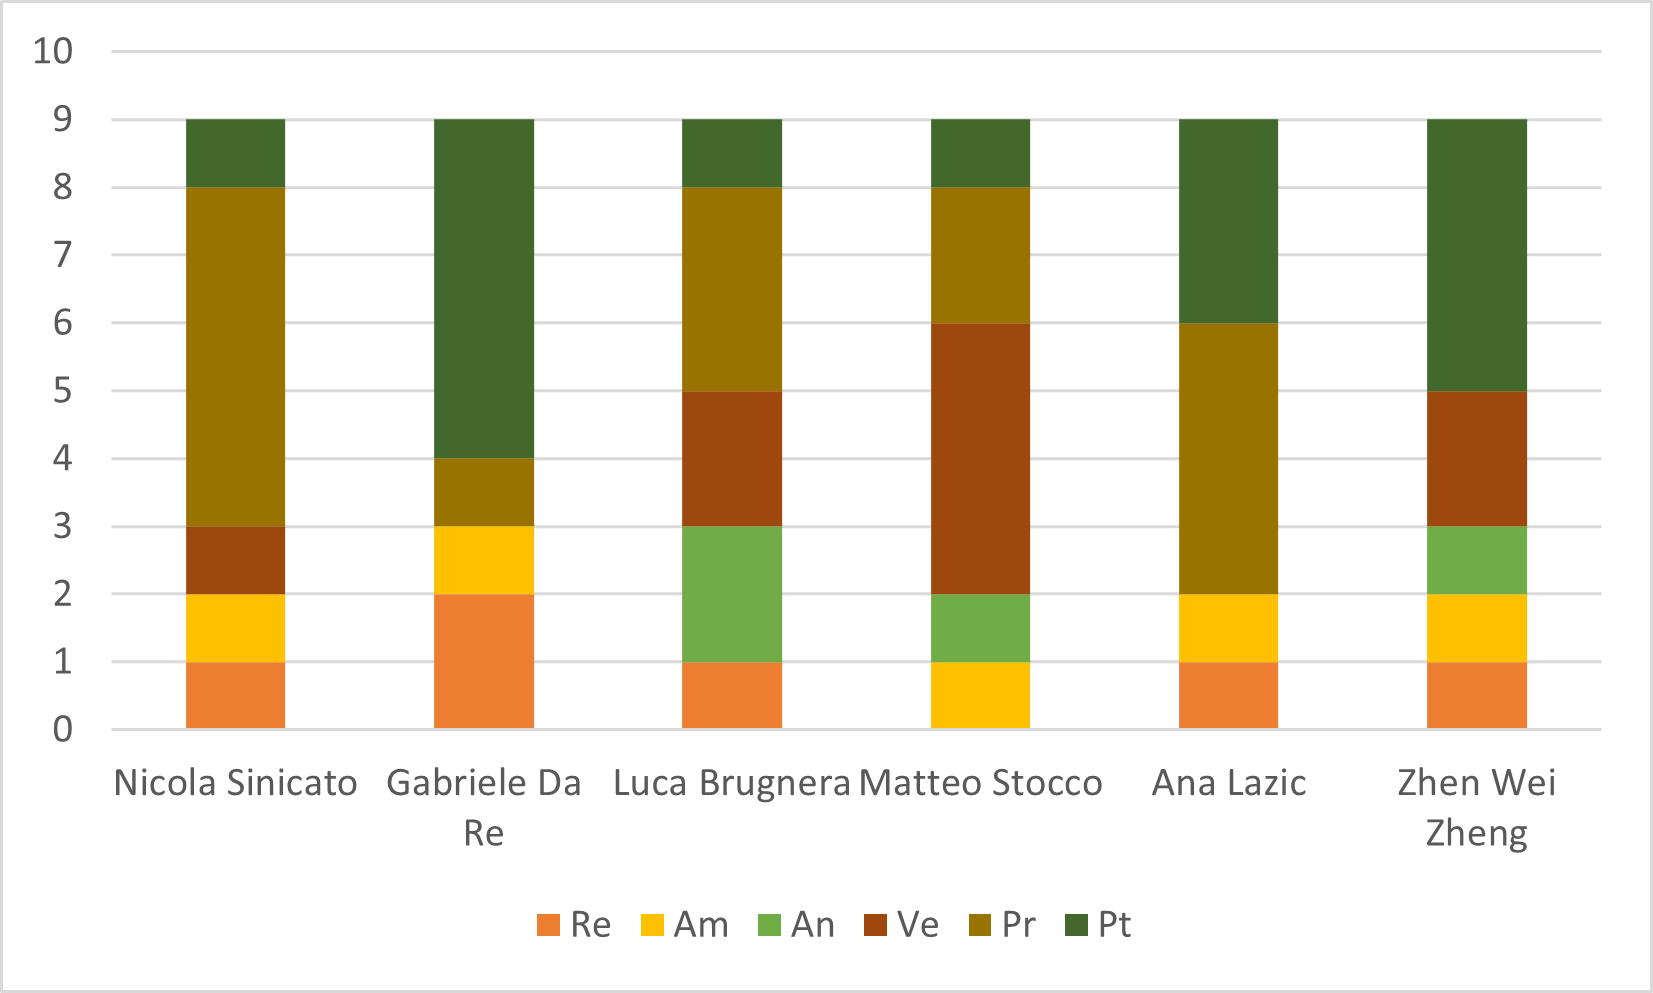
\includegraphics[scale=0.6]{img/grafi preventivo/istogrammi/proof/complessivo.png}
    \caption{Istogramma con la ripartizione delle ore nel periodo di produzione del proof of concept}
\end{figure}
\begin{figure}[H]
    \centering
    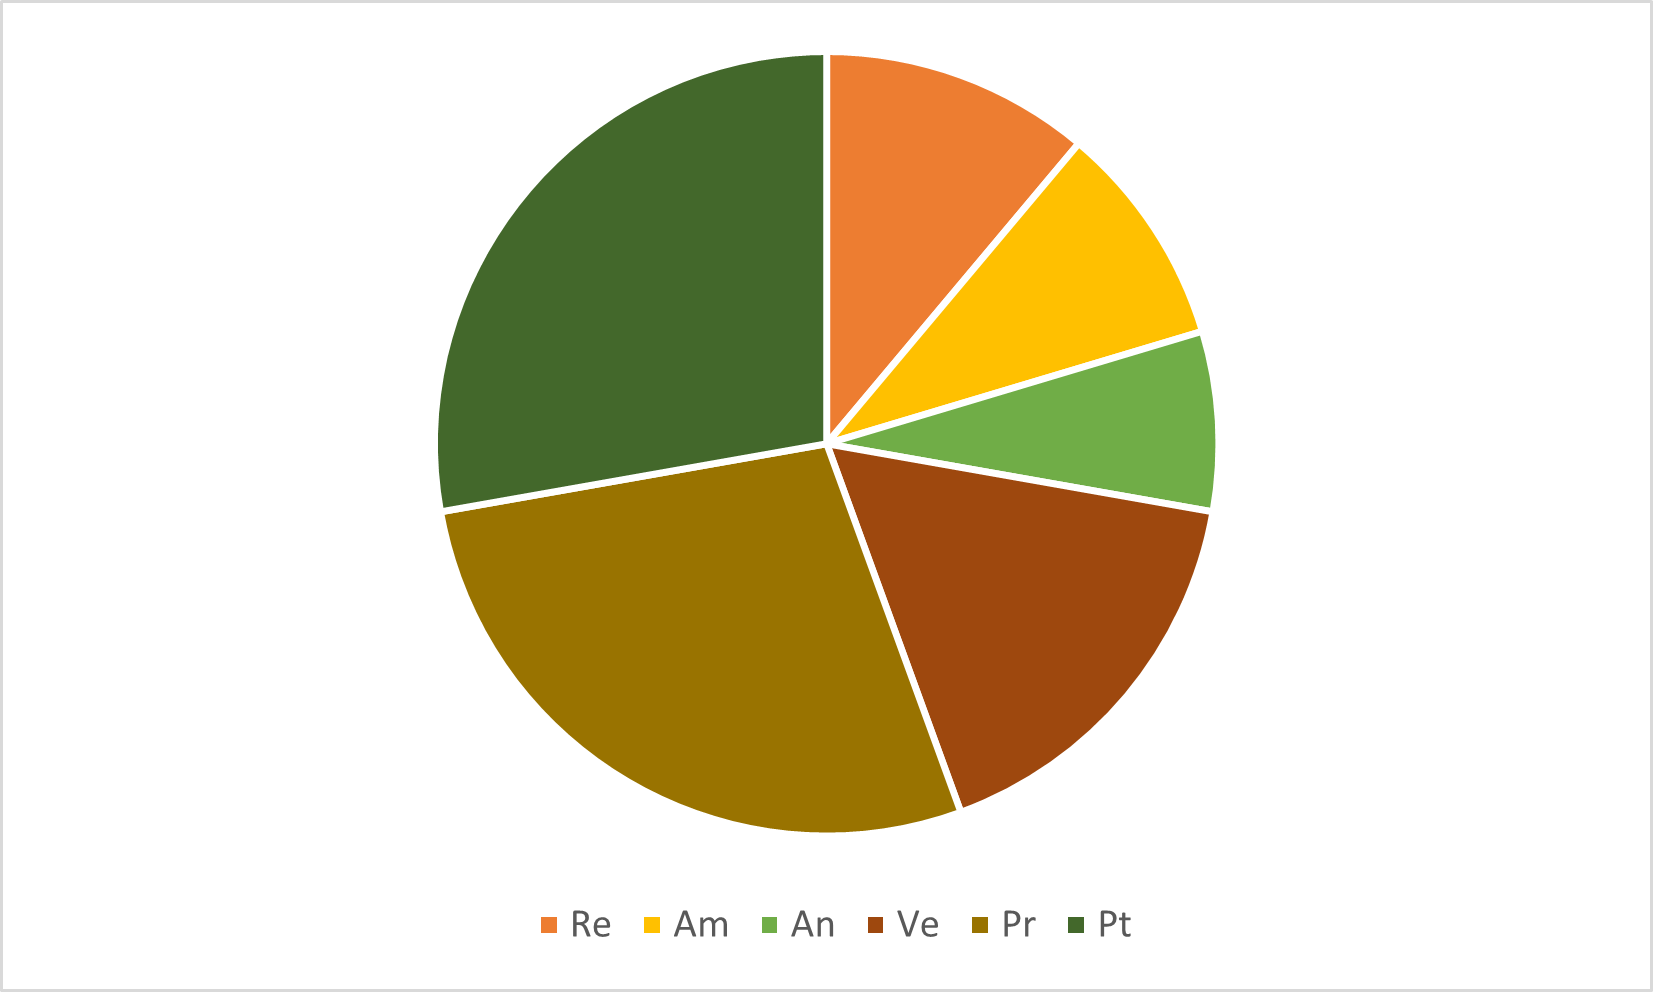
\includegraphics[scale=0.6]{img/grafi preventivo/torta/proof/complessivo.png}
    \caption{Grafico a torta con la ripartizione delle ore per ruolo nel periodo di produzione del proof of concept}
\end{figure}
\subsubsubsection{Preventivo dei costi}
La seguente tabella rappresenta le ore dedicate ad ogni ruolo e il corrispettivo costo in euro per il periodo di produzione del proof of concept:

	\setlength\extrarowheight{5pt}
	\rowcolors{2}{gray!10}{gray!40}
	\begin{tabularx}{\textwidth}{|ccc|c|}
		\hline
		\rowcolor{white}
		\textbf{Ruolo} & \textbf{Costo orario (€)} & \textbf{Ore totali} & \textbf{Costo totale (€)} \\
		\hline
		Responsabile &30&6&180 \\
		Amministratore &20&5&100 \\
		Analista &25&4&100 \\
		Verificatore &15&9&135 \\
		Programmatore &15&15&225 \\
		Progettista &25&15&375 \\
		\hline
		Totale &-&-&1115 \\
		\hline
		\rowcolor{white}
		\caption{Prospetto del costo orario durante il periodo di produzione del proof of concept per ruolo}
	\end{tabularx}
    \vspace{10pt}
	
% ----------------------------------------------------------------------------------------------------------------
%
\newpage
\subsection{Progettazione architetturale}

% ----------------------------------------------------------------------------------------------------------------
\subsubsection{Sprint\textsubscript{G} VII e riepilogo del periodo di progettazione architetturale}
% ----------------------------------------------------------------------------------------------------------------
%
\subsubsubsection{Preventivo orario}
La seguente tabella rappresenta la distribuzione oraria di ogni membro del gruppo per il settimo sprint\textsubscript{G} del progetto, il quale essendo l'unico a svolgersi durante il periodo di progettazione architetturale ha anche lo scopo di riepilogo per quest'ultimo:

	\setlength\extrarowheight{5pt}
	\rowcolors{2}{gray!10}{gray!40}
	\begin{tabularx}{\textwidth}{|ccccccc|c|}
		\hline
		\rowcolor{white}
		\textbf{Nome} & \textbf{Re} & \textbf{Am} & \textbf{An} & \textbf{Ve} & \textbf{Pr}& \textbf{Pt} & \textbf{Ore totali} \\
		\hline
		Nicola Sinicato &1&2&1&0&0&7&11 \\
		Gabriele Da Re &1&1&0&3&0&6&11 \\
		Luca Brugnera &1&2&1&0&0&7&11 \\
		Matteo Stocco &1&1&0&4&0&5&11 \\
		Ana Lazic &1&1&1&1&0&7&11 \\
		Zhen Wei Zheng &1&1&0&2&0&7&11 \\
		\hline
		Ore totali ruolo &6&8&3&10&0&39&66 \\
		\hline
		\rowcolor{white}
		\caption{Distribuzione oraria durante il periodo di progettazione architetturale per ruolo e persona}
	\end{tabularx}
	\vspace{10pt}
	
	\begin{figure}[H]
		\centering
		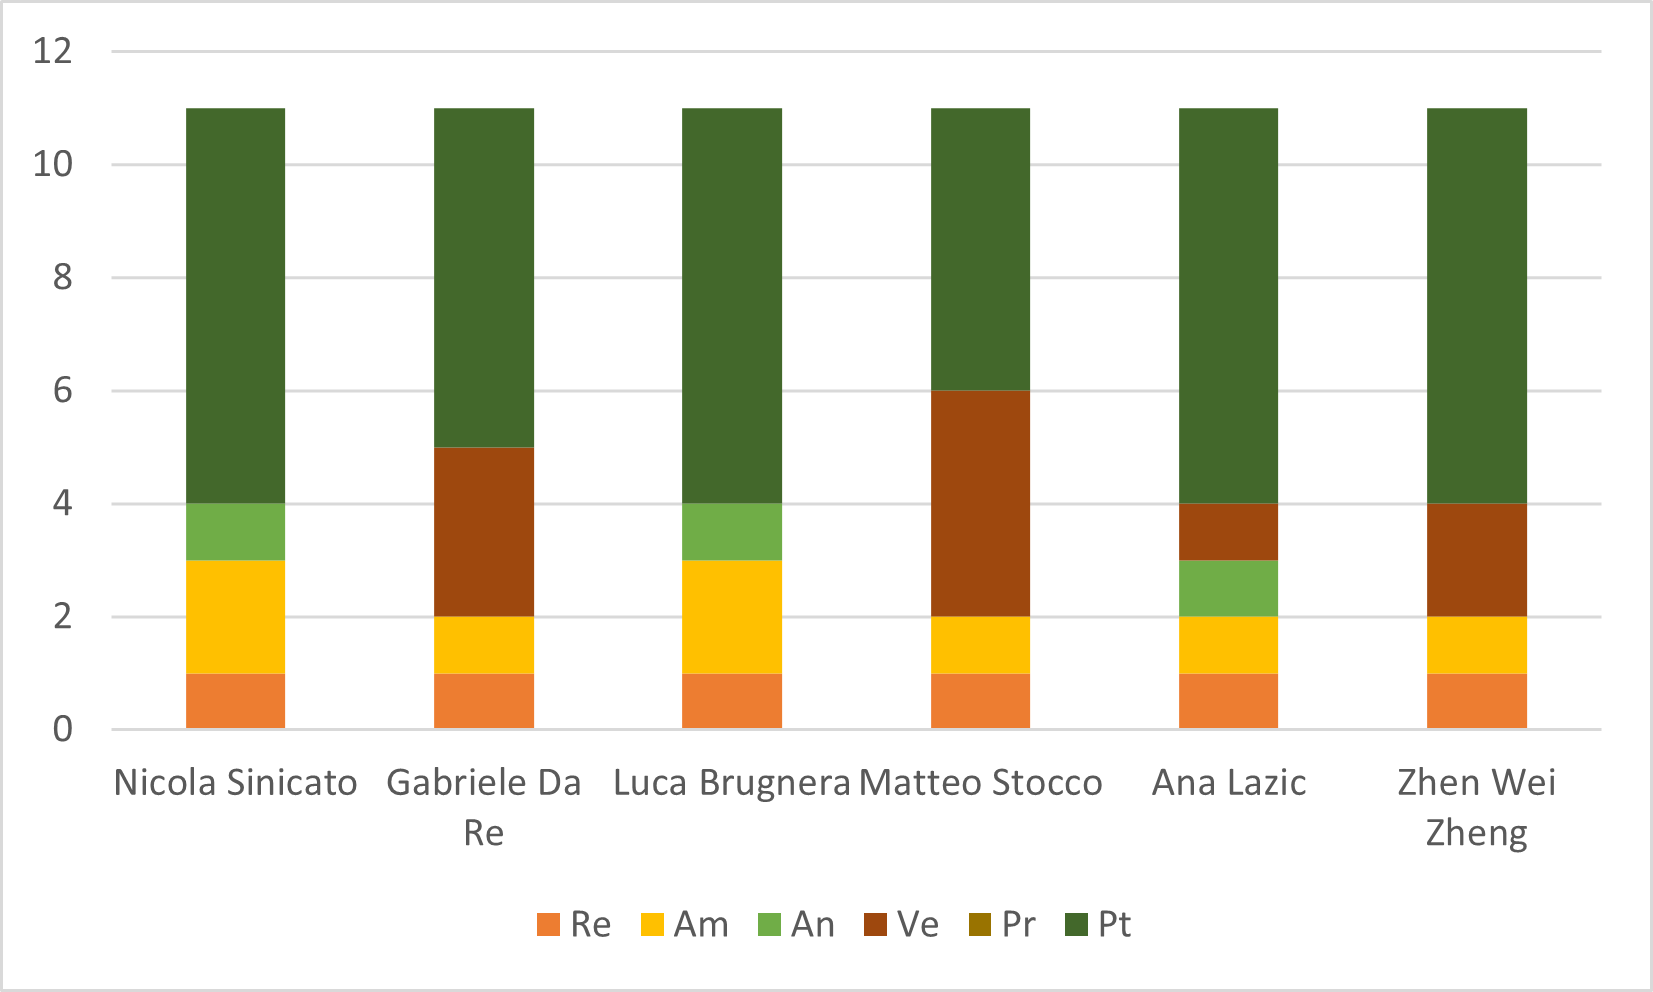
\includegraphics[scale=0.6]{img/grafi preventivo/istogrammi/architetturale/complessivo.png}
		\caption{Istogramma con la ripartizione delle ore nel periodo di progettazione architetturale}
	\end{figure}
	\begin{figure}[H]
		\centering
		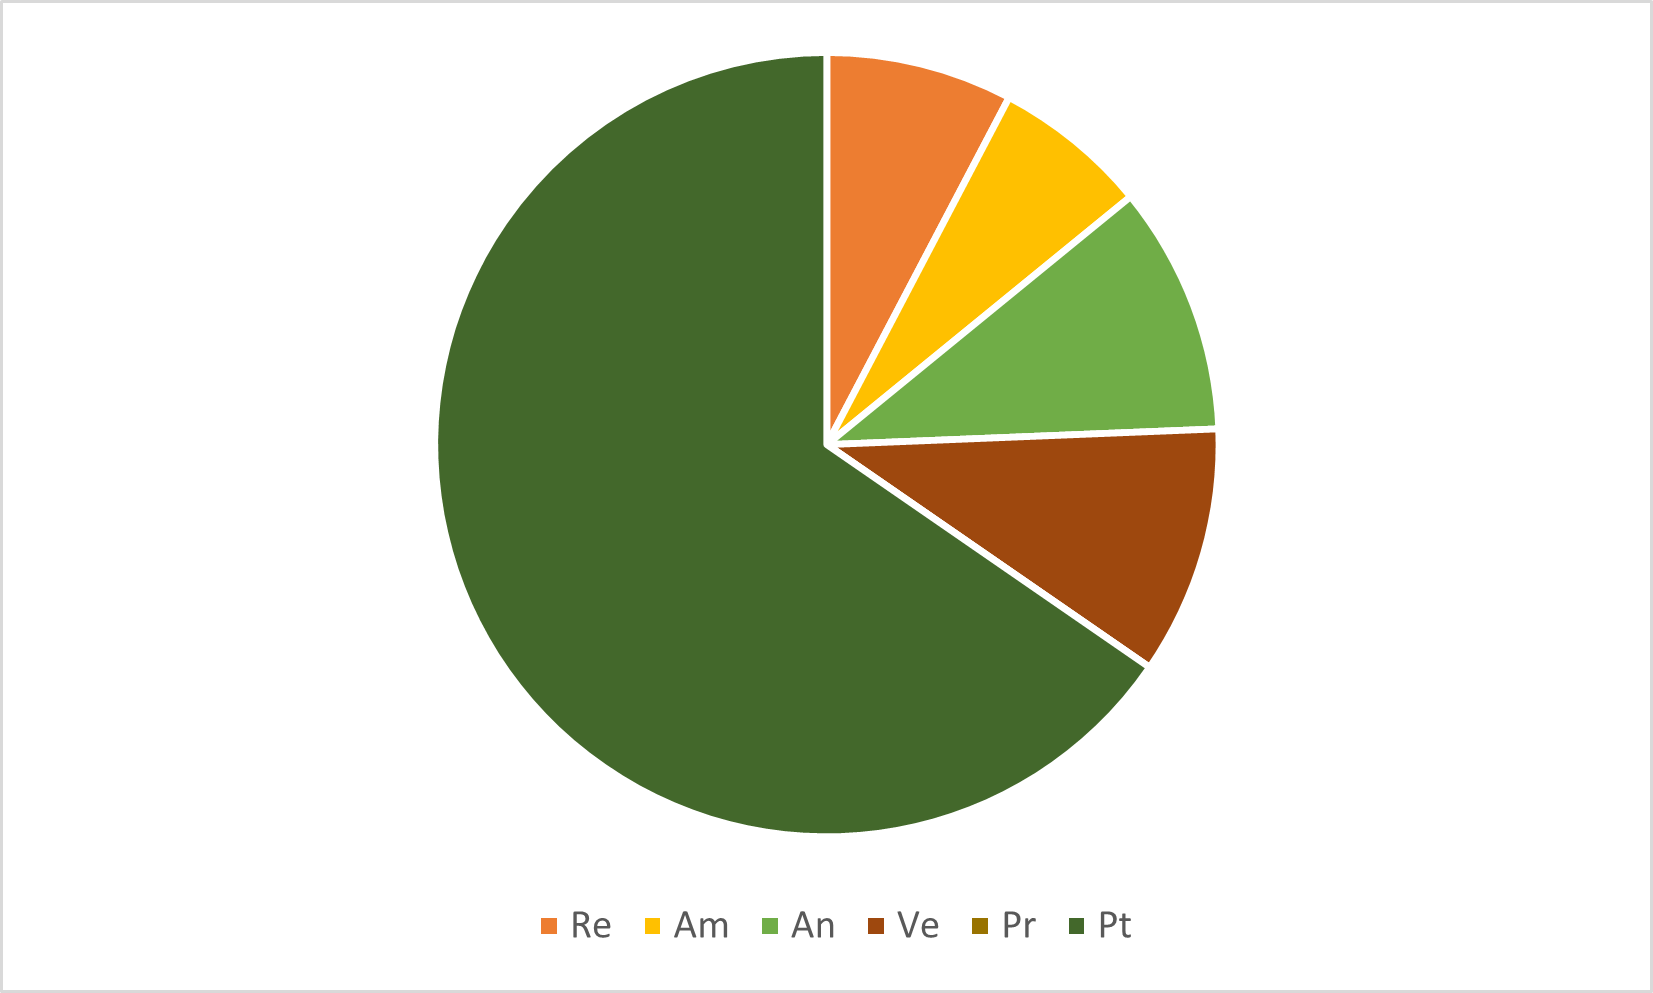
\includegraphics[scale=0.6]{img/grafi preventivo/torta/architetturale/complessivo.png}
		\caption{Grafico a torta con la ripartizione delle ore per ruolo nel periodo di progettazione architetturale}
	\end{figure}
	\subsubsubsection{Preventivo dei costi}
	La seguente tabella rappresenta le ore dedicate ad ogni ruolo e il corrispettivo costo in euro per il settimo sprint\textsubscript{G} del progetto, che ha anche lo scopo di riepilogo per il periodo di progettazione architetturale:
	
	\setlength\extrarowheight{5pt}
	\rowcolors{2}{gray!10}{gray!40}
	\begin{tabularx}{\textwidth}{|ccc|c|}
		\hline
		\rowcolor{white}
		\textbf{Ruolo} & \textbf{Costo orario (€)} & \textbf{Ore totali} & \textbf{Costo totale (€)} \\
		\hline
		Responsabile &30&6&180 \\
		Amministratore &20&8&160 \\
		Analista &25&3&75 \\
		Verificatore &15&10&150 \\
		Programmatore &15&0&0 \\
		Progettista &25&39&975 \\
		\hline
		Totale &-&-&1540 \\
		\hline
		\rowcolor{white}
		\caption{Prospetto del costo orario durante il periodo di progettazione architetturale per ruolo}
	\end{tabularx}
	\vspace{10pt}
% ----------------------------------------------------------------------------------------------------------------
\newpage
\subsection{Progettazione di dettaglio e codifica}
% ----------------------------------------------------------------------------------------------------------------
\subsubsection{Sprint\textsubscript{G} VIII}
% ----------------------------------------------------------------------------------------------------------------
%
\subsubsubsection{Preventivo orario}
La seguente tabella rappresenta la distribuzione oraria di ogni membro del gruppo per l'ottavo sprint\textsubscript{G} del progetto, il quale è svolto nel periodo di progettazione di dettaglio e codifica:

	\setlength\extrarowheight{5pt}
	\rowcolors{2}{gray!10}{gray!40}
	\begin{tabularx}{\textwidth}{|ccccccc|c|}
		\hline
		\rowcolor{white}
		\textbf{Nome} & \textbf{Re} & \textbf{Am} & \textbf{An} & \textbf{Ve} & \textbf{Pr}& \textbf{Pt} & \textbf{Ore totali} \\
		\hline
		Nicola Sinicato &1&1&0&0&1&3&6 \\
		Gabriele Da Re &0&0&0&0&2&4&6 \\
		Luca Brugnera &1&1&0&2&0&2&6 \\
		Matteo Stocco &1&0&0&1&0&4&6 \\
		Ana Lazic &0&0&0&0&2&4&6 \\
		Zhen Wei Zheng &0&1&0&2&1&2&6 \\
		\hline
		Ore totali ruolo &3&3&0&5&6&19&36 \\
		\hline
		\rowcolor{white}
		\caption{Distribuzione oraria durante l'ottavo sprint\textsubscript{G} per ruolo e persona}
	\end{tabularx}
	\vspace{10pt}
	
\begin{figure}[H]
    \centering
    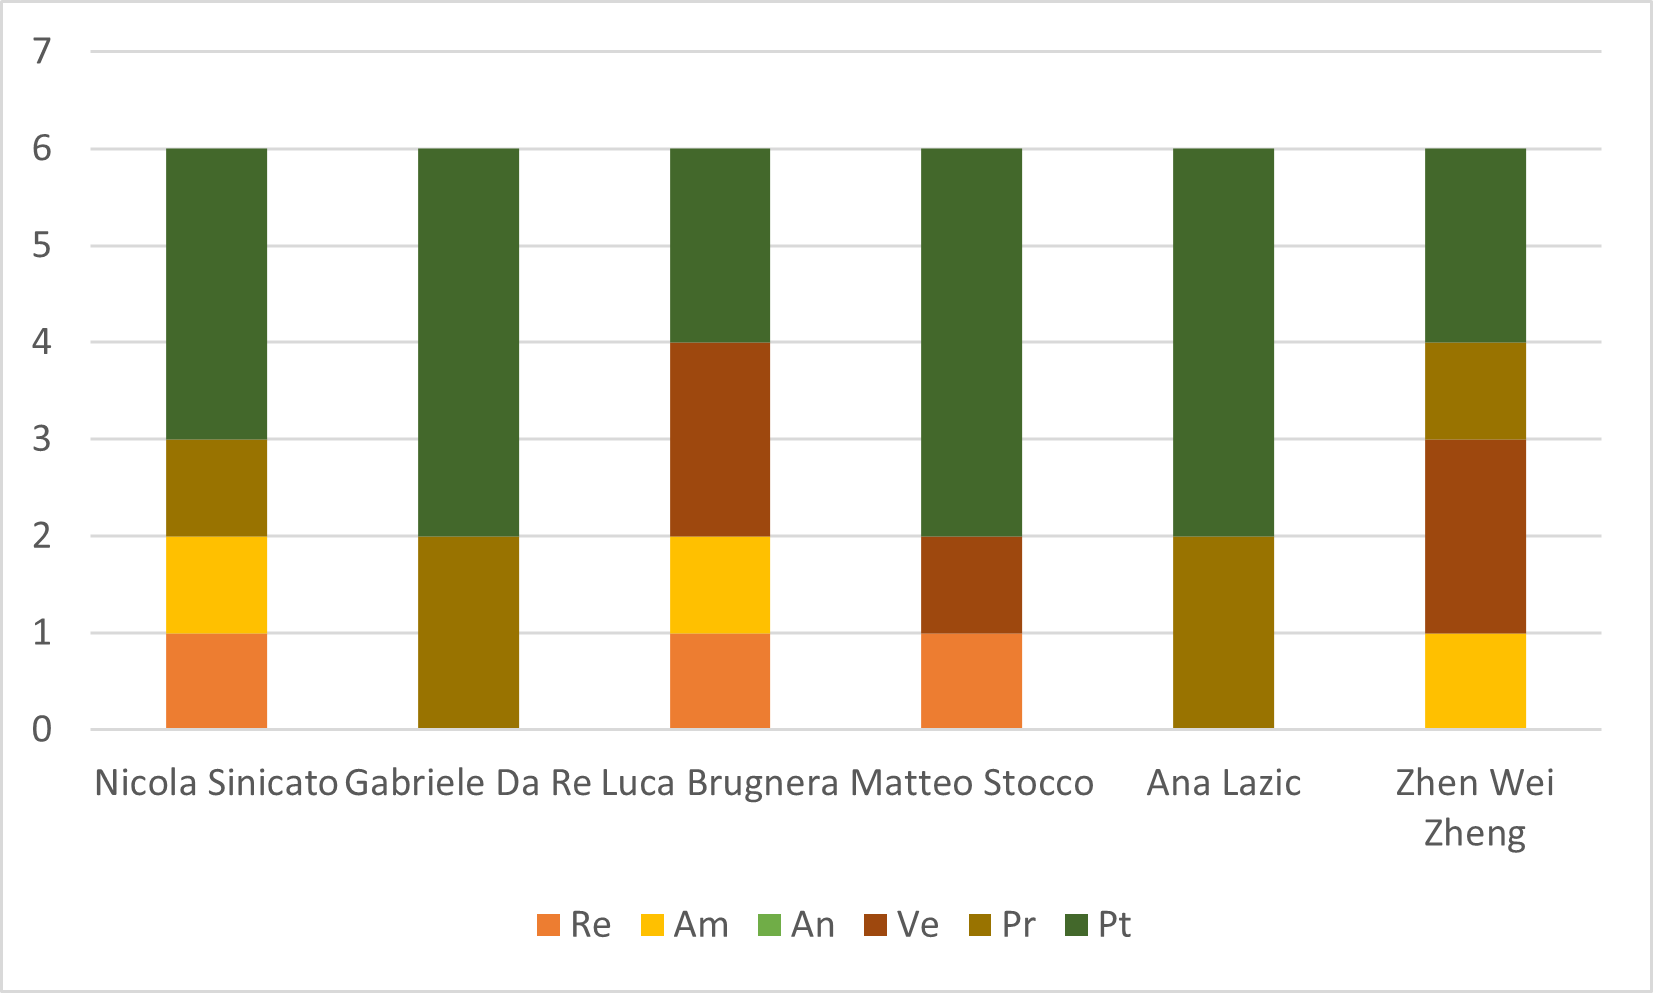
\includegraphics[scale=0.6]{img/grafi preventivo/istogrammi/codifica/sprint8.png}
    \caption{Istogramma con la ripartizione delle ore dell'ottavo sprint\textsubscript{G}}
\end{figure}
\begin{figure}[H]
    \centering
    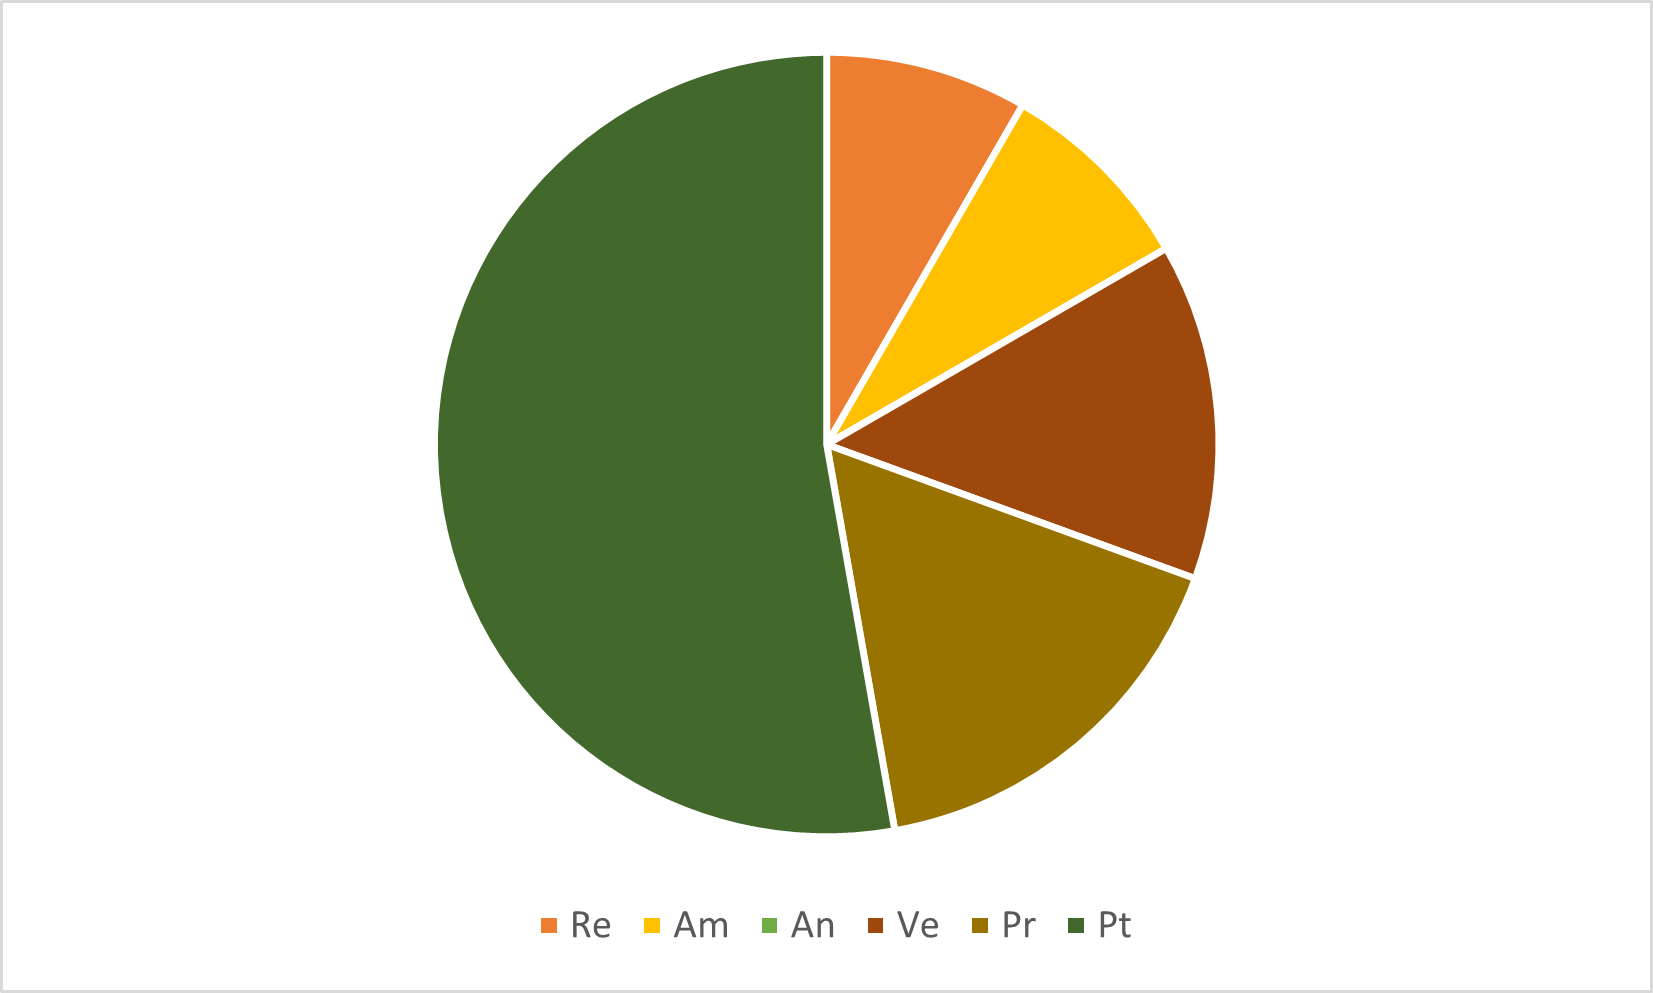
\includegraphics[scale=0.6]{img/grafi preventivo/torta/codifica/sprint8.png}
    \caption{Grafico a torta con la ripartizione delle ore per ruolo nell'ottavo sprint\textsubscript{G}}
\end{figure}
\subsubsubsection{Preventivo dei costi}
La seguente tabella rappresenta le ore dedicate ad ogni ruolo e il corrispettivo costo in euro per l'ottavo sprint\textsubscript{G}, svolto nel periodo di progettazione di dettaglio e codifica: 

	\setlength\extrarowheight{5pt}
	\rowcolors{2}{gray!10}{gray!40}
	\begin{tabularx}{\textwidth}{|ccc|c|}
		\hline
		\rowcolor{white}
		\textbf{Ruolo} & \textbf{Costo orario (€)} & \textbf{Ore totali} & \textbf{Costo totale (€)} \\
		\hline
		Responsabile &30&3&90 \\
		Amministratore &20&3&60 \\
		Analista &25&0&0 \\
		Verificatore &15&5&75 \\
		Programmatore &15&6&90 \\
		Progettista &25&19&475 \\
		\hline
		Totale &-&-&790 \\
		\hline
		\rowcolor{white}
		\caption{Prospetto del costo orario durante l'ottavo sprint\textsubscript{G} per ruolo}
	\end{tabularx}
    \vspace{10pt}
	
%
% ----------------------------------------------------------------------------------------------------------------
\newpage
\subsubsection{Sprint\textsubscript{G} IX}
% ----------------------------------------------------------------------------------------------------------------
%
\subsubsubsection{Preventivo orario}
La seguente tabella rappresenta la distribuzione oraria di ogni membro del gruppo per il nono sprint\textsubscript{G} del progetto, il quale è svolto nel periodo di progettazione di dettaglio e codifica:

	\setlength\extrarowheight{5pt}
	\rowcolors{2}{gray!10}{gray!40}
	\begin{tabularx}{\textwidth}{|ccccccc|c|}
		\hline
		\rowcolor{white}
		\textbf{Nome} & \textbf{Re} & \textbf{Am} & \textbf{An} & \textbf{Ve} & \textbf{Pr}& \textbf{Pt} & \textbf{Ore totali} \\
		\hline
		Nicola Sinicato &0&0&0&3&9&0&12 \\
		Gabriele Da Re &1&1&0&1&8&1&12 \\
		Luca Brugnera &0&1&0&1&9&1&12 \\
		Matteo Stocco &0&0&0&2&9&0&11 \\
		Ana Lazic &1&1&0&1&7&1&11 \\
		Zhen Wei Zheng &0&2&0&2&8&0&12 \\
		\hline
		Ore totali ruolo &2&5&0&10&50&3&70 \\
		\hline
		\rowcolor{white}
		\caption{Distribuzione oraria durante il nono sprint\textsubscript{G} per ruolo e persona}
	\end{tabularx}
	\vspace{10pt}
	
\begin{figure}[H]
    \centering
    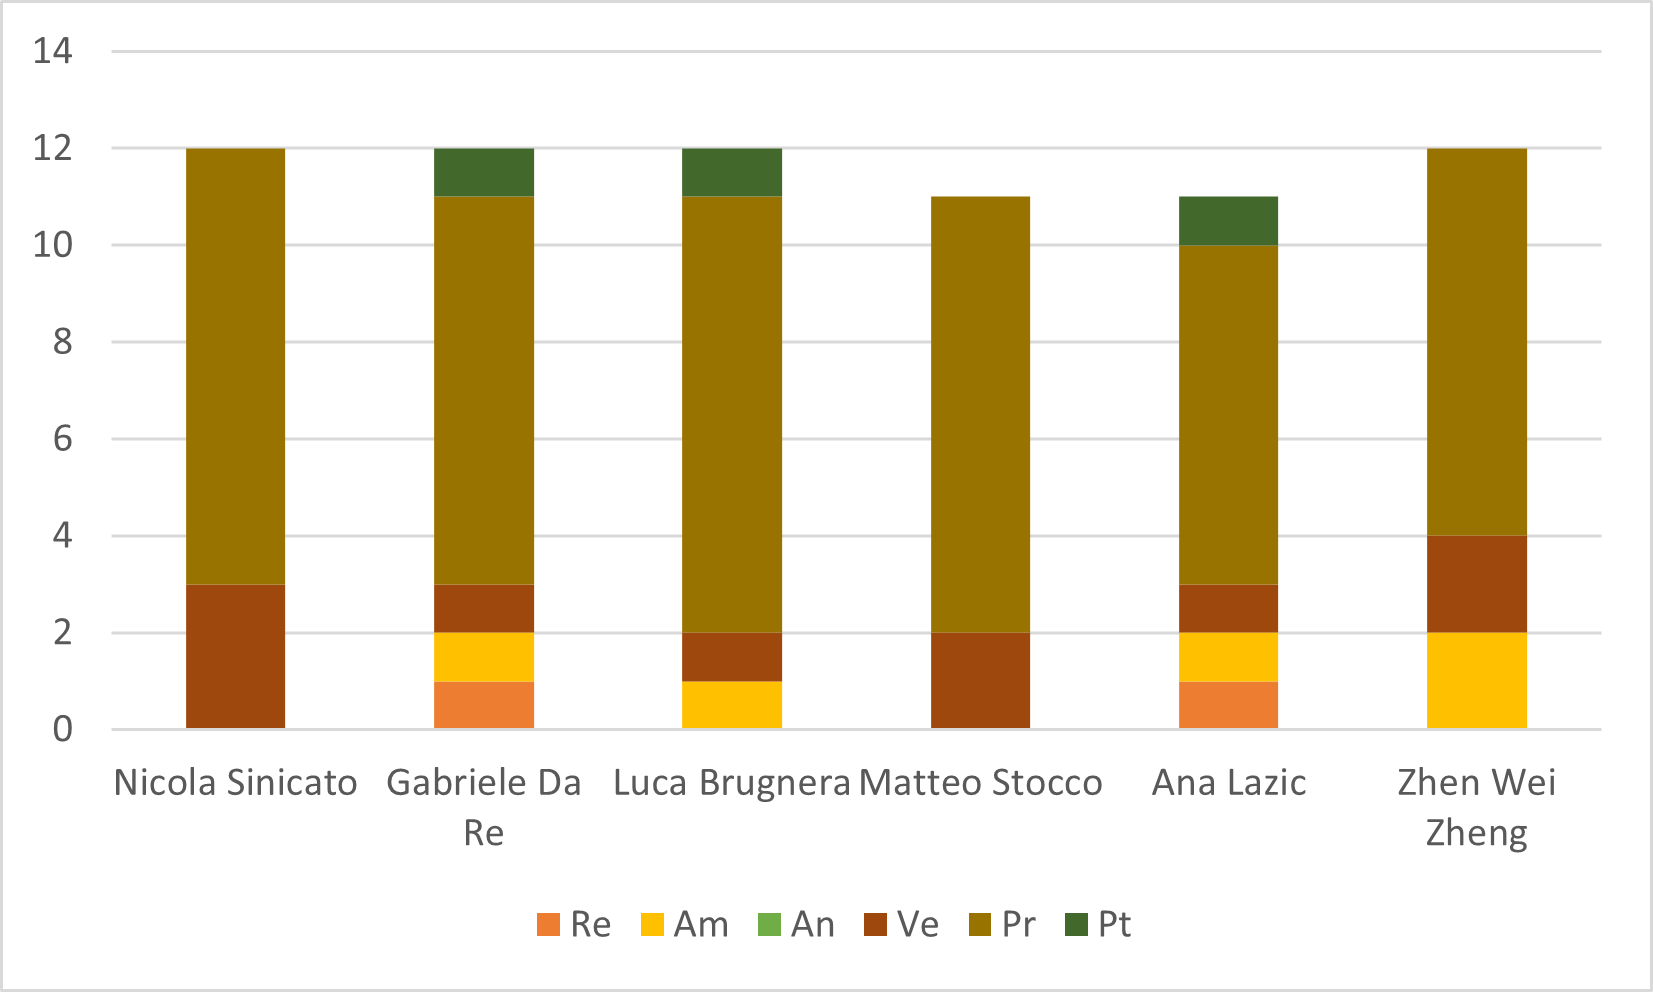
\includegraphics[scale=0.6]{img/grafi preventivo/istogrammi/codifica/sprint9.png}
    \caption{Istogramma con la ripartizione delle ore del nono sprint\textsubscript{G}}
\end{figure}
\begin{figure}[H]
    \centering
    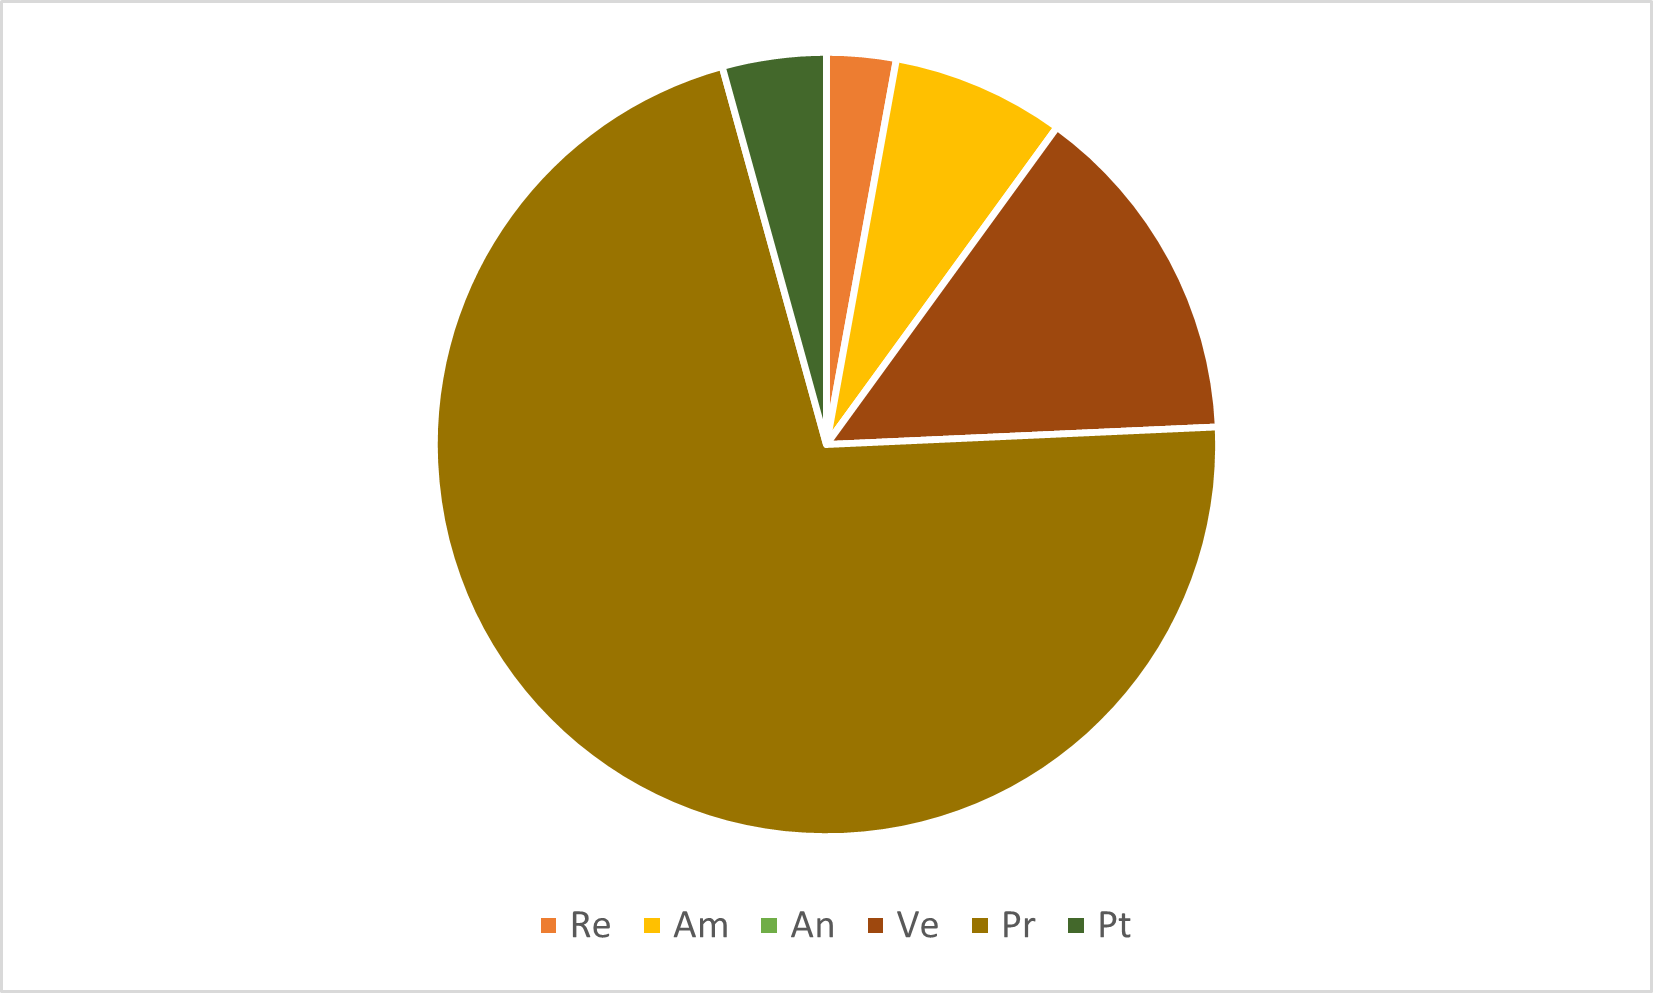
\includegraphics[scale=0.6]{img/grafi preventivo/torta/codifica/sprint9.png}
    \caption{Grafico a torta con la ripartizione delle ore per ruolo nel nono sprint\textsubscript{G}}
\end{figure}
\subsubsubsection{Preventivo dei costi}
La seguente tabella rappresenta le ore dedicate ad ogni ruolo e il corrispettivo costo in euro per il nono sprint\textsubscript{G}, svolto nel periodo di progettazione di dettaglio e codifica: 

	\setlength\extrarowheight{5pt}
	\rowcolors{2}{gray!10}{gray!40}
	\begin{tabularx}{\textwidth}{|ccc|c|}
		\hline
		\rowcolor{white}
		\textbf{Ruolo} & \textbf{Costo orario (€)} & \textbf{Ore totali} & \textbf{Costo totale (€)} \\
		\hline
		Responsabile &30&2&60 \\
		Amministratore &20&5&100 \\
		Analista &25&0&0 \\
		Verificatore &15&10&150 \\
		Programmatore &15&50&750 \\
		Progettista &25&3&75 \\
		\hline
		Totale &-&-&1135 \\
		\hline
		\rowcolor{white}
		\caption{Prospetto del costo orario durante il nono sprint\textsubscript{G} per ruolo}
	\end{tabularx}
    \vspace{10pt}
	
%
% ----------------------------------------------------------------------------------------------------------------

%
% ----------------------------------------------------------------------------------------------------------------
\newpage
\subsubsection{Sprint\textsubscript{G} X}
% ----------------------------------------------------------------------------------------------------------------
%
\subsubsubsection{Preventivo orario}
La seguente tabella rappresenta la distribuzione oraria di ogni membro del gruppo per il decimo sprint\textsubscript{G} del progetto, il quale è svolto nel periodo di progettazione di dettaglio e codifica:

\setlength\extrarowheight{5pt}
\rowcolors{2}{gray!10}{gray!40}
\begin{tabularx}{\textwidth}{|ccccccc|c|}
	\hline
	\rowcolor{white}
	\textbf{Nome} & \textbf{Re} & \textbf{Am} & \textbf{An} & \textbf{Ve} & \textbf{Pr}& \textbf{Pt} & \textbf{Ore totali} \\
	\hline
	Nicola Sinicato &0&0&0&1&4&0&5 \\
	Gabriele Da Re &0&1&0&0&4&1&5 \\
	Luca Brugnera &0&0&0&1&3&1&5 \\
	Matteo Stocco &0&0&0&2&3&0&5 \\
	Ana Lazic &0&0&0&1&4&0&5 \\
	Zhen Wei Zheng &1&0&0&1&3&0&5 \\
	\hline
	Ore totali ruolo &1&1&0&6&21&1&30 \\
	\hline
	\rowcolor{white}
	\caption{Distribuzione oraria durante il decimo sprint\textsubscript{G} per ruolo e persona}
\end{tabularx}
\vspace{10pt}

\begin{figure}[H]
	\centering
	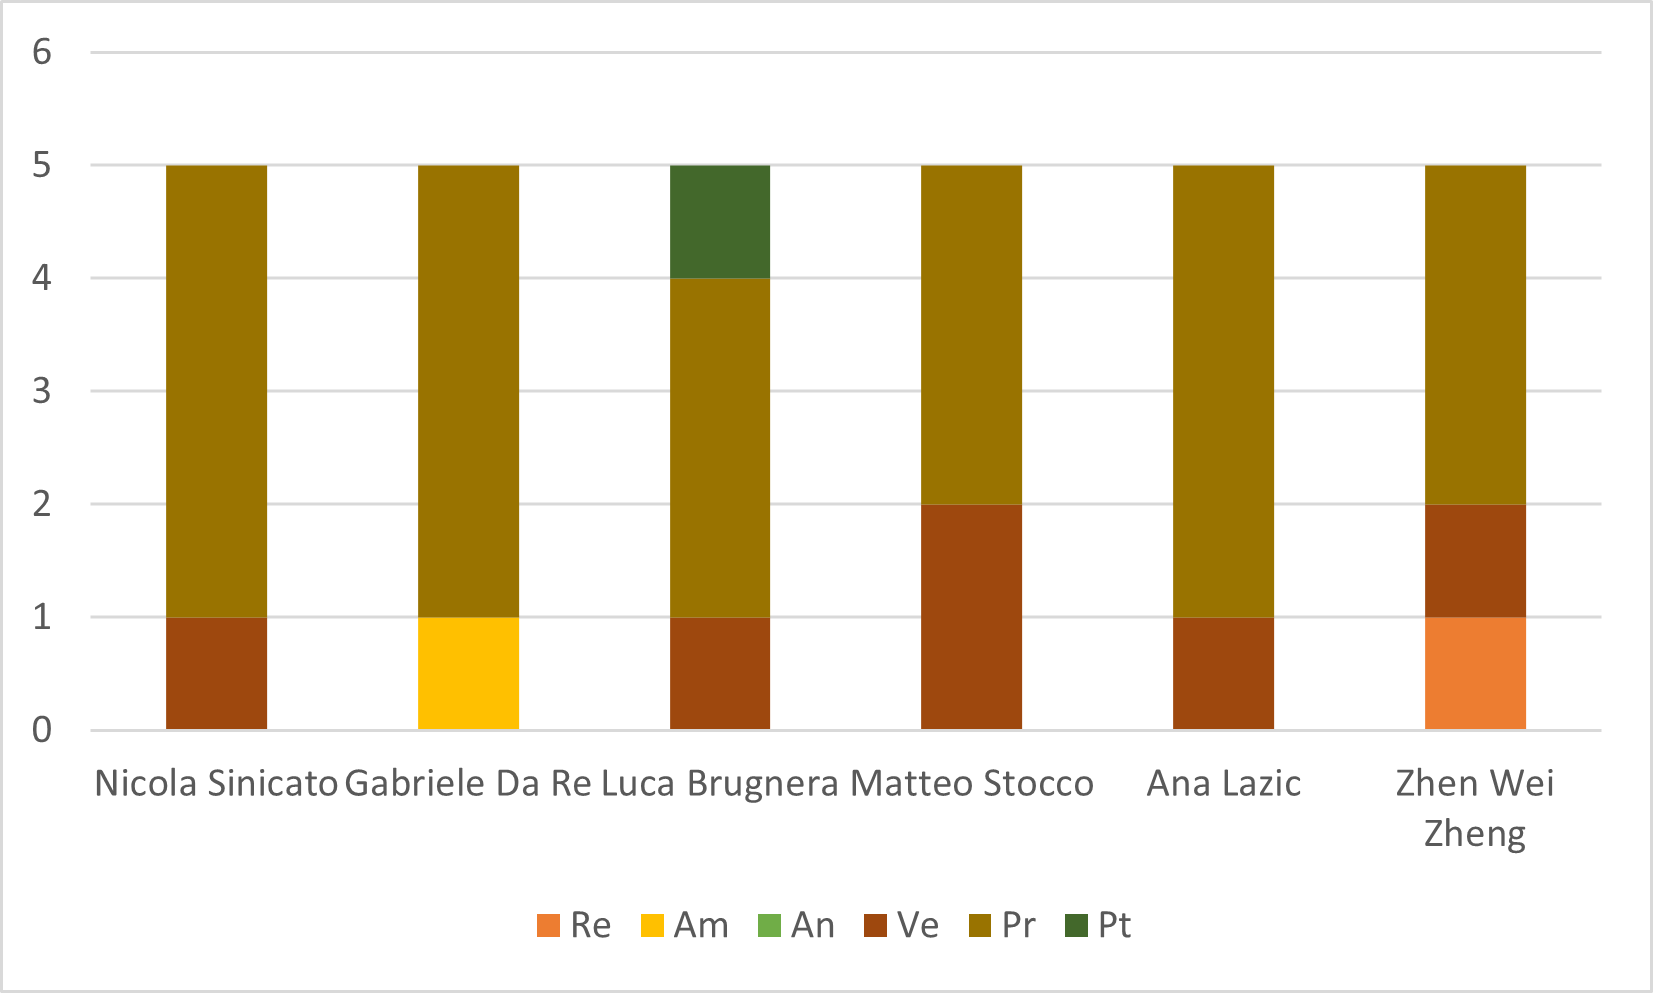
\includegraphics[scale=0.6]{img/grafi preventivo/istogrammi/codifica/sprint10.png}
	\caption{Istogramma con la ripartizione delle ore del decimo sprint\textsubscript{G}}
\end{figure}
\begin{figure}[H]
	\centering
	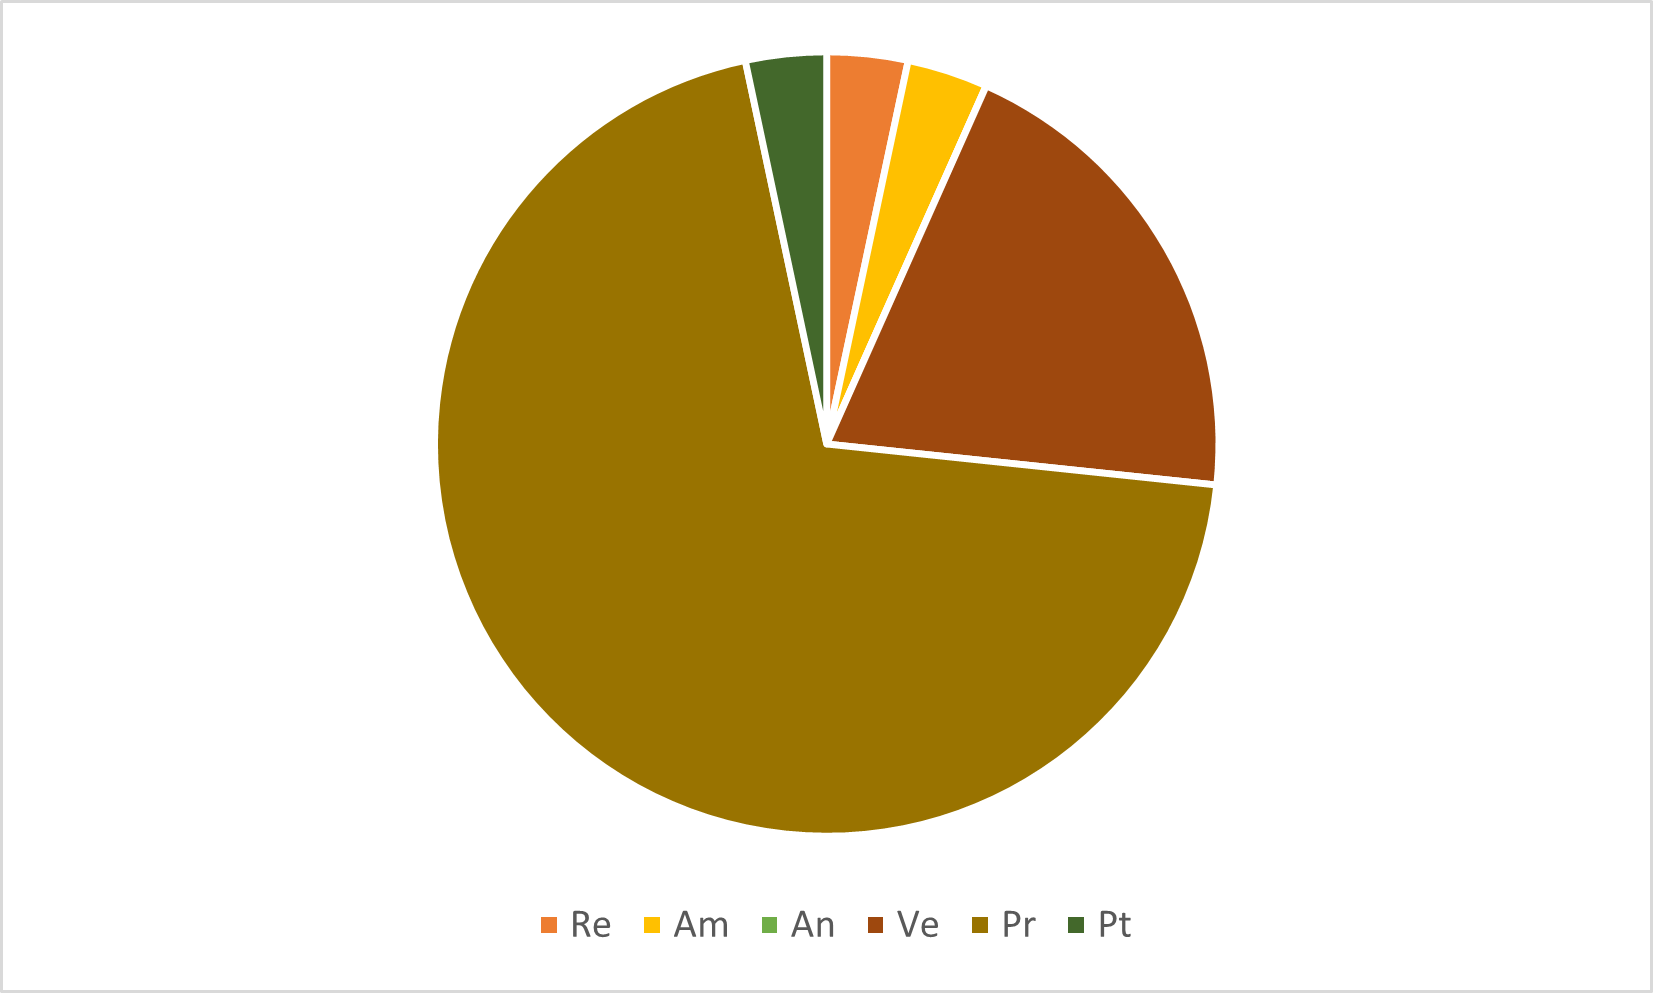
\includegraphics[scale=0.6]{img/grafi preventivo/torta/codifica/sprint10.png}
	\caption{Grafico a torta con la ripartizione delle ore per ruolo nel decimo sprint\textsubscript{G}}
\end{figure}
\subsubsubsection{Preventivo dei costi}
La seguente tabella rappresenta le ore dedicate ad ogni ruolo e il corrispettivo costo in euro per il decimo sprint\textsubscript{G}, svolto nel periodo di progettazione di dettaglio e codifica: 

\setlength\extrarowheight{5pt}
\rowcolors{2}{gray!10}{gray!40}
\begin{tabularx}{\textwidth}{|ccc|c|}
	\hline
	\rowcolor{white}
	\textbf{Ruolo} & \textbf{Costo orario (€)} & \textbf{Ore totali} & \textbf{Costo totale (€)} \\
	\hline
	Responsabile &30&1&30 \\
	Amministratore &20&1&20 \\
	Analista &25&0&0 \\
	Verificatore &15&6&90 \\
	Programmatore &15&21&315 \\
	Progettista &25&1&25 \\
	\hline
	Totale &-&-&480 \\
	\hline
	\rowcolor{white}
	\caption{Prospetto del costo orario durante il decimo sprint\textsubscript{G} per ruolo}
\end{tabularx}
% ----------------------------------------------------------------------------------------------------------------
\newpage

\subsubsection{Riepilogo del periodo di progettazione di dettaglio e codifica}
% ----------------------------------------------------------------------------------------------------------------
%
\subsubsubsection{Preventivo orario}
La seguente tabella rappresenta la distribuzione oraria per ogni membro del gruppo per il periodo di progettazione di dettaglio e codifica:

	\setlength\extrarowheight{5pt}
	\rowcolors{2}{gray!10}{gray!40}
	\begin{tabularx}{\textwidth}{|ccccccc|c|}
		\hline
		\rowcolor{white}
		\textbf{Nome} & \textbf{Re} & \textbf{Am} & \textbf{An} & \textbf{Ve} & \textbf{Pr}& \textbf{Pt} & \textbf{Ore totali} \\
		\hline
		Nicola Sinicato &1&1&0&4&14&3&23 \\
		Gabriele Da Re &1&2&0&1&14&5&23 \\
		Luca Brugnera &1&2&0&4&12&4&23 \\
		Matteo Stocco &1&0&0&5&12&4&22 \\
		Ana Lazic &1&1&0&2&13&5&22 \\
		Zhen Wei Zheng &1&3&0&5&12&2&23 \\
		\hline
		Ore totali ruolo &6&9&0&21&77&33&136 \\
		\hline
		\rowcolor{white}
		\caption{Distribuzione oraria durante il periodo di progettazione di dettaglio e codifica per ruolo e persona}
	\end{tabularx}
	\vspace{10pt}
	
\begin{figure}[H]
    \centering
    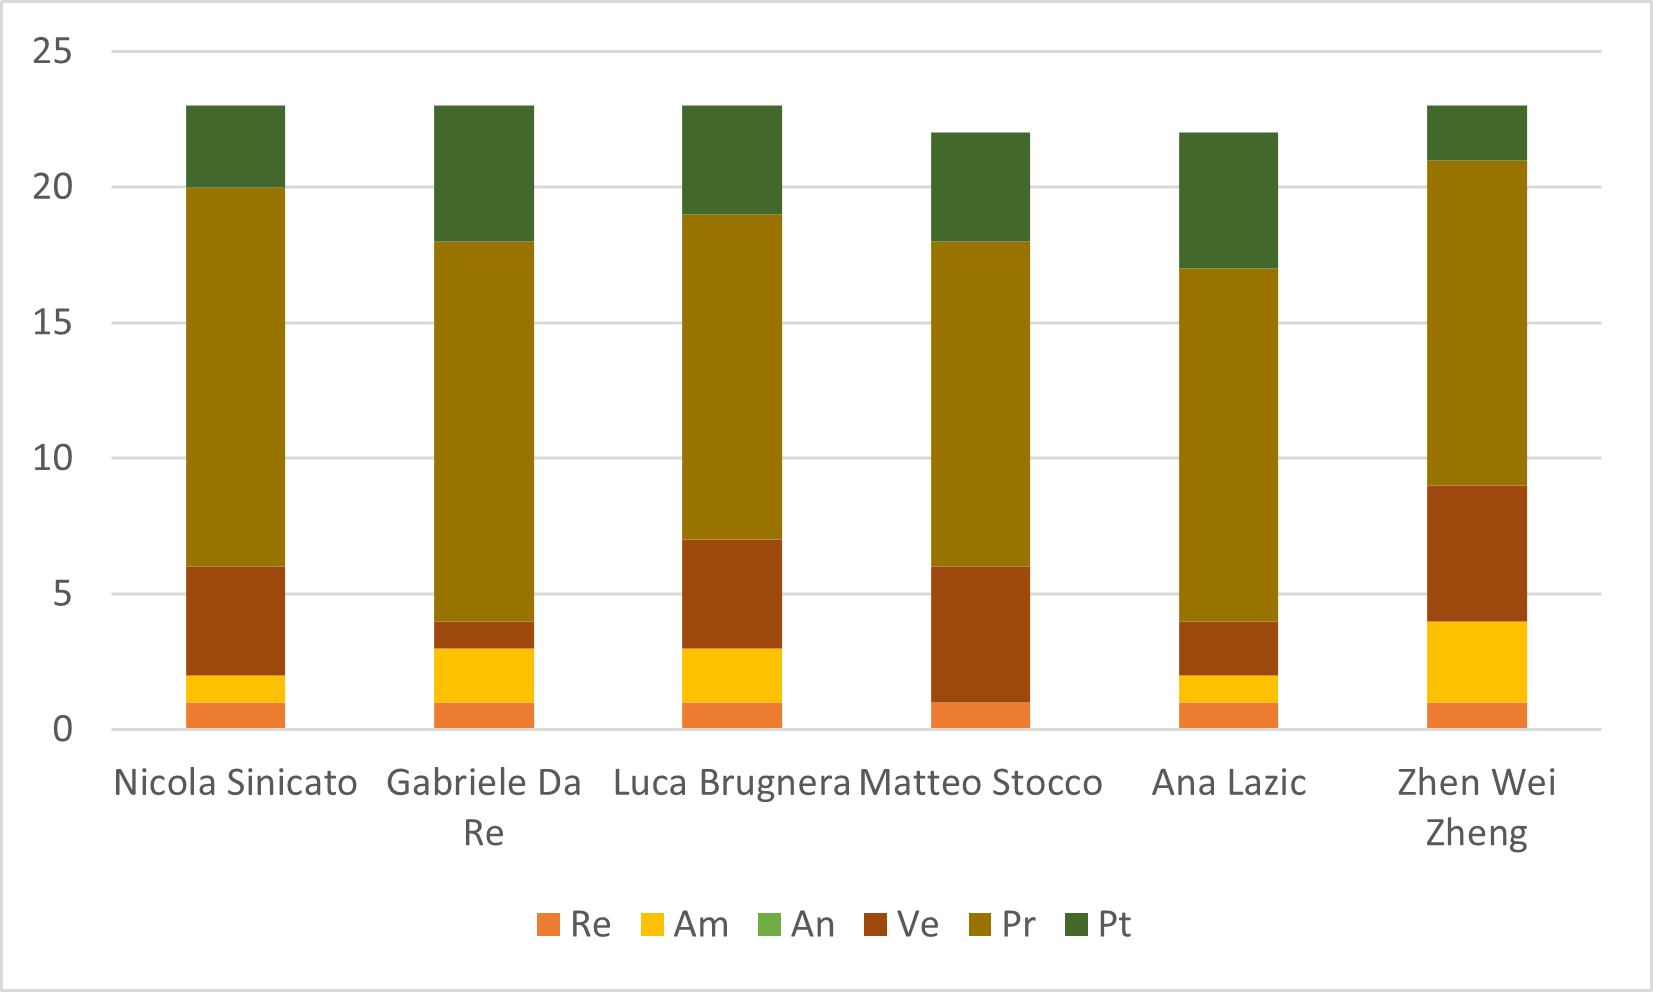
\includegraphics[scale=0.6]{img/grafi preventivo/istogrammi/codifica/complessivo.png}
    \caption{Istogramma con la ripartizione delle ore nel periodo di progettazione di dettaglio e codifica}
\end{figure}
\begin{figure}[H]
    \centering
    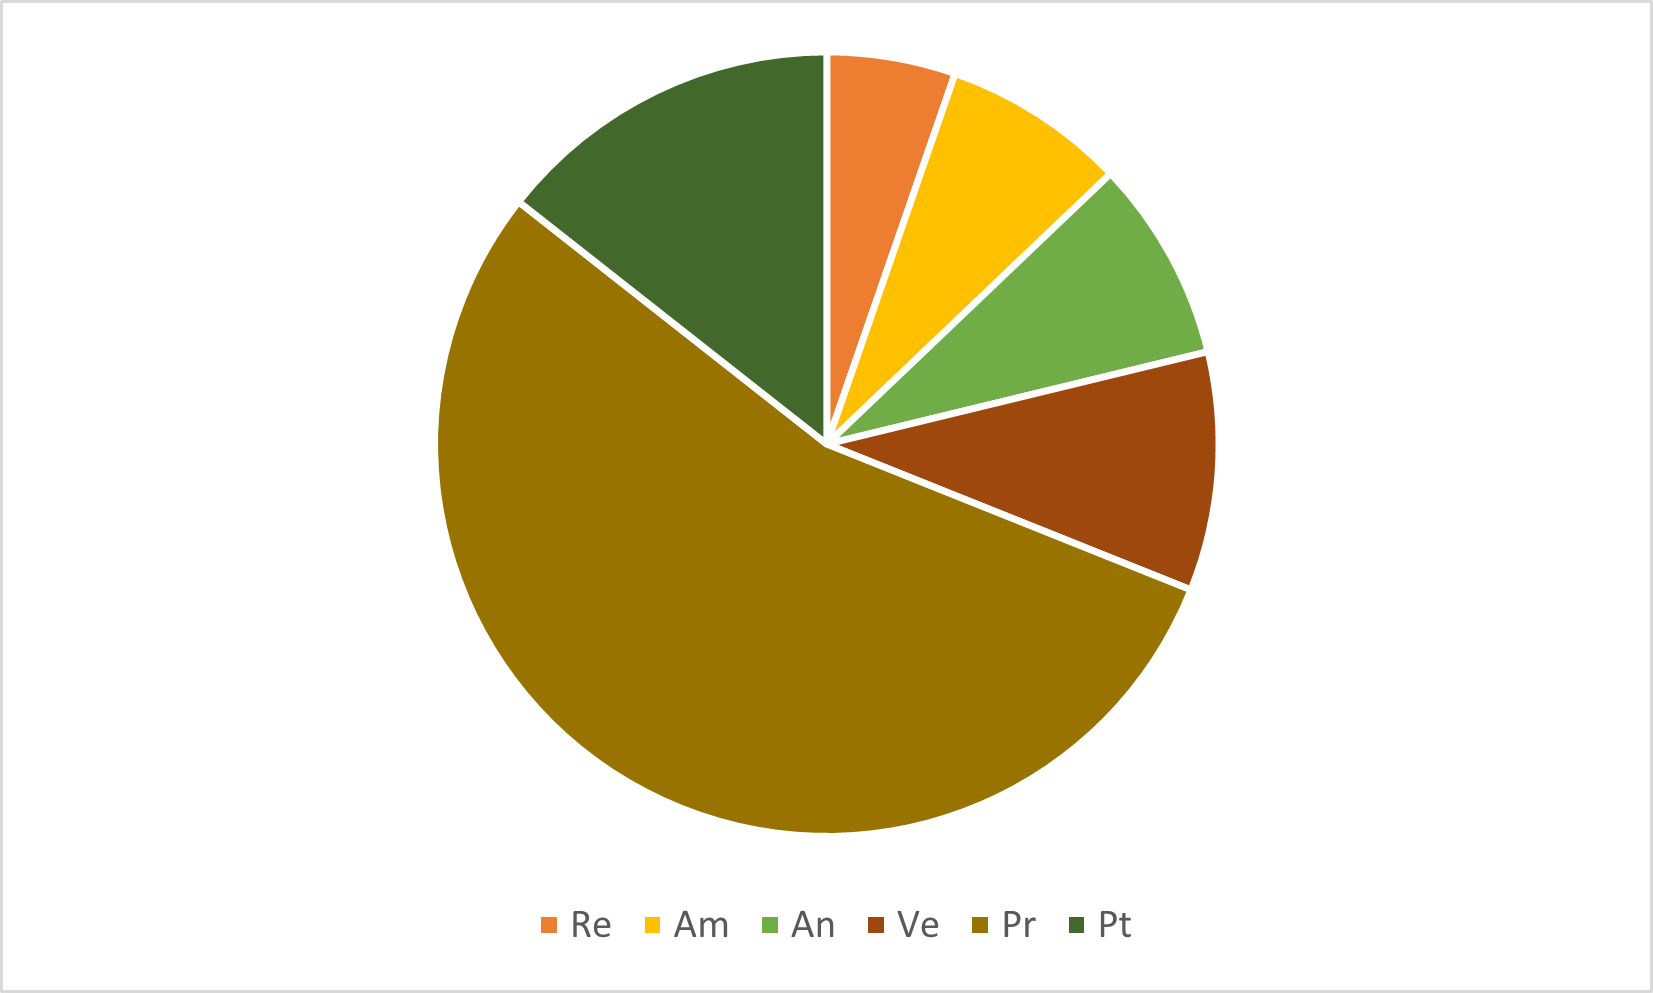
\includegraphics[scale=0.6]{img/grafi preventivo/torta/codifica/complessivo.png}
    \caption{Grafico a torta con la ripartizione delle ore per ruolo nel periodo di progettazione di dettaglio e codifica}
\end{figure}
\subsubsubsection{Preventivo dei costi}
La seguente tabella rappresenta le ore dedicate ad ogni ruolo e il corrispettivo costo in euro per il periodo di progettazione di dettaglio e codifica:

	\setlength\extrarowheight{5pt}
	\rowcolors{2}{gray!10}{gray!40}
	\begin{tabularx}{\textwidth}{|ccc|c|}
		\hline
		\rowcolor{white}
		\textbf{Ruolo} & \textbf{Costo orario (€)} & \textbf{Ore totali} & \textbf{Costo totale (€)} \\
		\hline
		Responsabile &30&6&180 \\
		Amministratore &20&9&180 \\
		Analista &25&0&0 \\
		Verificatore &15&21&315 \\
		Programmatore &15&77&1155 \\
		Progettista &25&23&575 \\
		\hline
		Totale &-&-&2405 \\
		\hline
		\rowcolor{white}
		\caption{Prospetto del costo orario durante il periodo di progettazione di dettaglio e codifica per ruolo}
	\end{tabularx}
    \vspace{10pt}
	
% ----------------------------------------------------------------------------------------------------------------
\newpage
\subsection{Validazione\textsubscript{G} e collaudo}
% ----------------------------------------------------------------------------------------------------------------
\subsubsection{Sprint\textsubscript{G} XI e riepilogo del periodo di validazione\textsubscript{G} e collaudo}
% ----------------------------------------------------------------------------------------------------------------
%
\subsubsubsection{Preventivo orario}
La seguente tabella rappresenta la distribuzione oraria di ogni membro del gruppo per l'undicesimo sprint\textsubscript{G} del progetto, il quale essendo l'unico a svolgersi durante il periodo di validazione\textsubscript{G} e collaudo ha anche lo scopo di riepilogo per quest'ultimo:

\setlength\extrarowheight{5pt}
\rowcolors{2}{gray!10}{gray!40}
\begin{tabularx}{\textwidth}{|ccccccc|c|}
	\hline
	\rowcolor{white}
	\textbf{Nome} & \textbf{Re} & \textbf{Am} & \textbf{An} & \textbf{Ve} & \textbf{Pr}& \textbf{Pt} & \textbf{Ore totali} \\
	\hline
	Nicola Sinicato &3&0&0&6&2&0&11 \\
	Gabriele Da Re &1&3&0&5&2&0&11 \\
	Luca Brugnera &0&2&0&7&2&0&11 \\
	Matteo Stocco &3&0&0&6&2&0&11 \\
	Ana Lazic &3&1&0&6&1&0&11 \\
	Zhen Wei Zheng &1&2&0&7&1&0&11 \\
	\hline
	Ore totali ruolo &11&8&0&37&10&0&66 \\
	\hline
	\rowcolor{white}
	\caption{Distribuzione oraria durante il periodo di validazione\textsubscript{G} e collaudo per ruolo e persona}
\end{tabularx}
\vspace{10pt}

\begin{figure}[H]
	\centering
	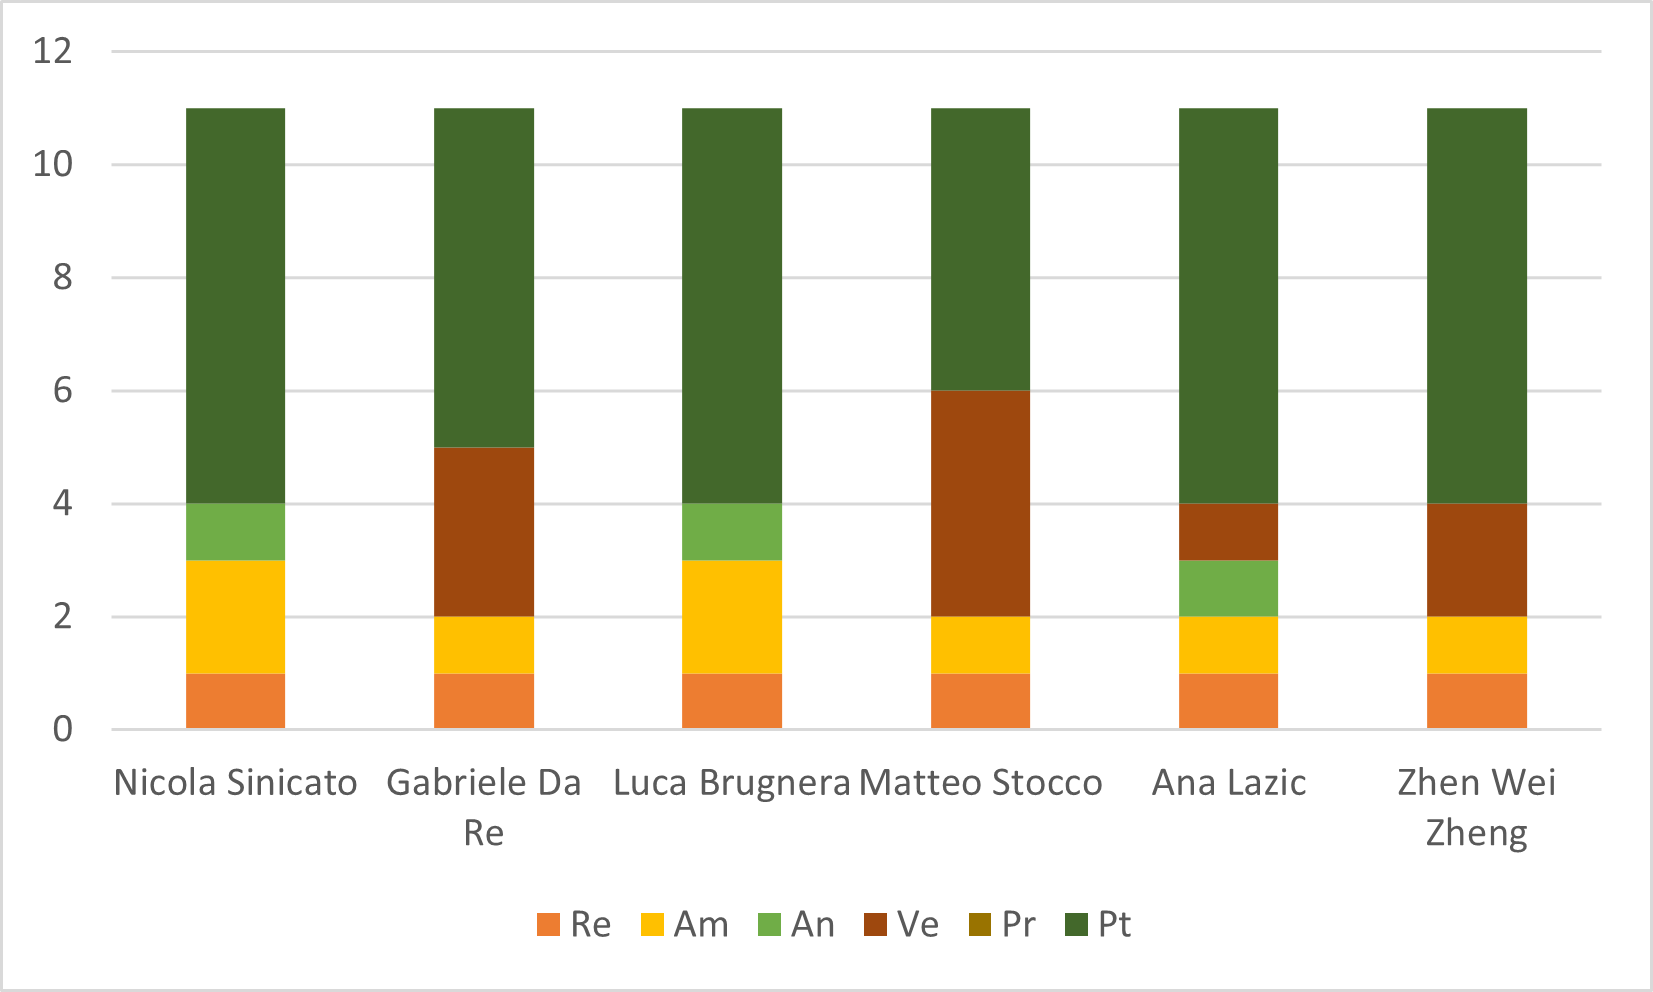
\includegraphics[scale=0.6]{img/grafi preventivo/istogrammi/architetturale/complessivo.png}
	\caption{Istogramma con la ripartizione delle ore nel periodo di validazione\textsubscript{G} e collaudo}
\end{figure}
\begin{figure}[H]
	\centering
	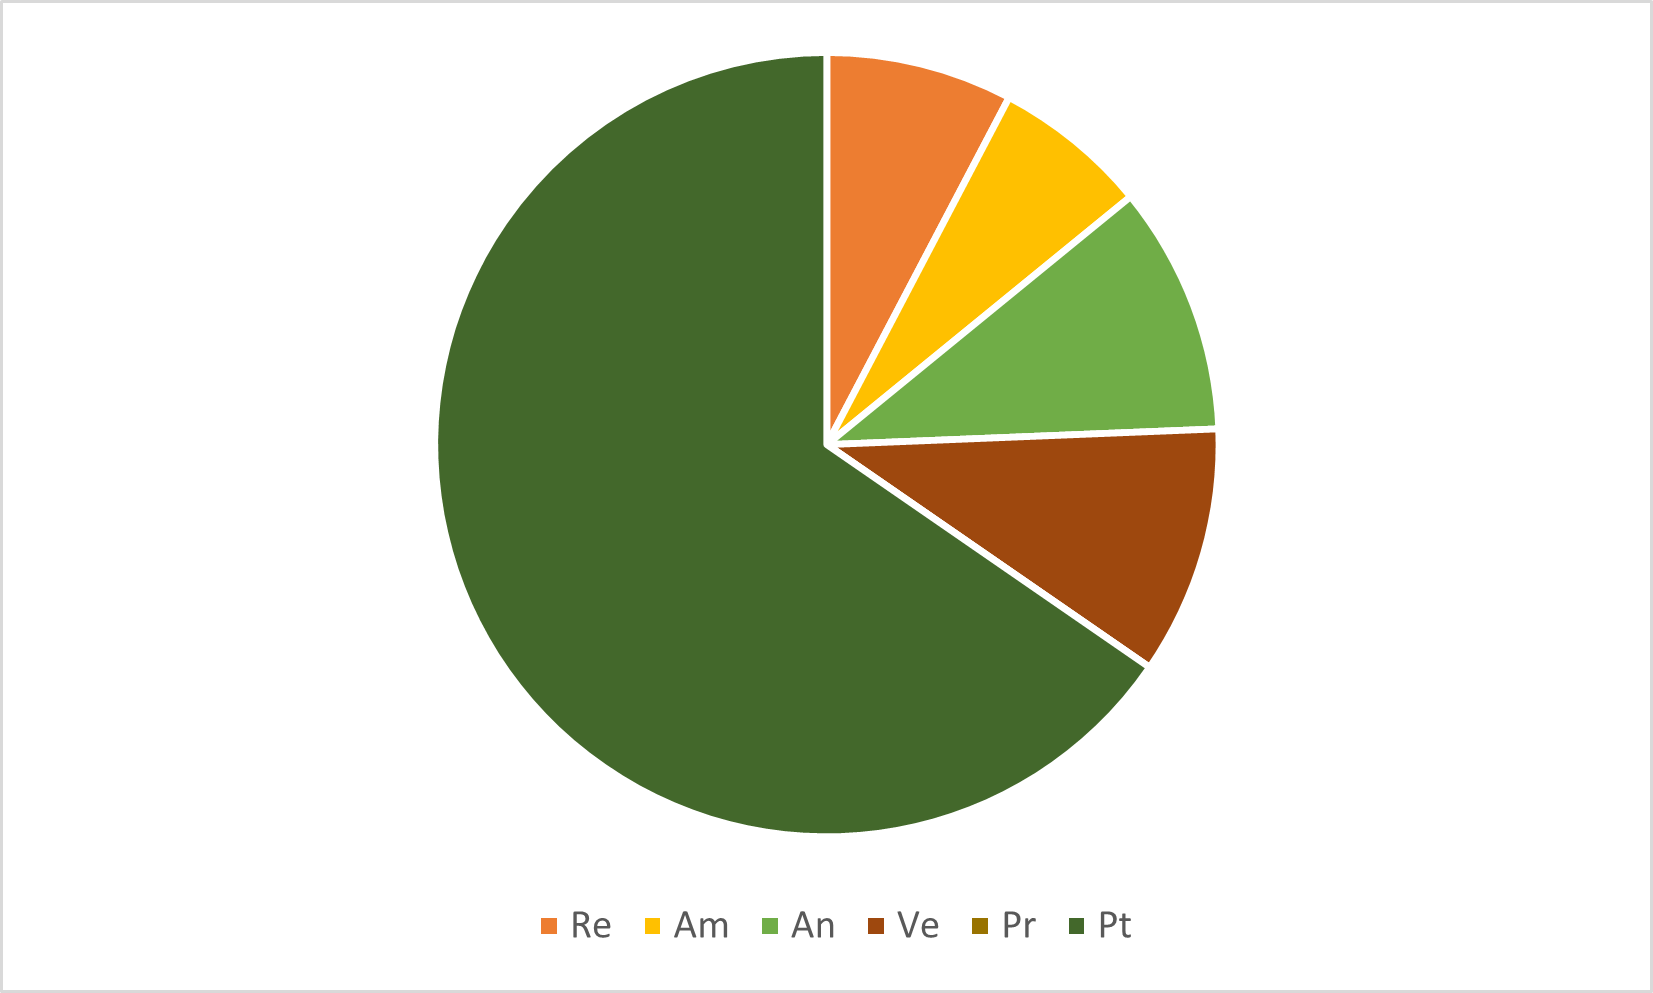
\includegraphics[scale=0.6]{img/grafi preventivo/torta/architetturale/complessivo.png}
	\caption{Grafico a torta con la ripartizione delle ore per ruolo nel periodo di validazione\textsubscript{G} e collaudo}
\end{figure}
\subsubsubsection{Preventivo dei costi}
La seguente tabella rappresenta le ore dedicate ad ogni ruolo e il corrispettivo costo in euro per l'undicesimo sprint\textsubscript{G} del progetto, che ha anche lo scopo di riepilogo per il periodo di validazione\textsubscript{G} e collaudo:

\setlength\extrarowheight{5pt}
\rowcolors{2}{gray!10}{gray!40}
\begin{tabularx}{\textwidth}{|ccc|c|}
	\hline
	\rowcolor{white}
	\textbf{Ruolo} & \textbf{Costo orario (€)} & \textbf{Ore totali} & \textbf{Costo totale (€)} \\
	\hline
	Responsabile &30&11&330 \\
	Amministratore &20&8&160 \\
	Analista &25&0&0 \\
	Verificatore &15&37&555 \\
	Programmatore &15&10&150 \\
	Progettista &25&0&0 \\
	\hline
	Totale &-&-&1195 \\
	\hline
	\rowcolor{white}
	\caption{Prospetto del costo orario durante il periodo di validazione\textsubscript{G} e collaudo per ruolo}
\end{tabularx}
% ----------------------------------------------------------------------------------------------------------------
\newpage
\subsection{Riepilogo complessivo}
% ----------------------------------------------------------------------------------------------------------------
%
\subsubsection{Preventivo orario}
La seguente tabella rappresenta la distribuzione oraria complessiva per ogni membro del gruppo:

	\setlength\extrarowheight{5pt}
	\rowcolors{2}{gray!10}{gray!40}
	\begin{tabularx}{\textwidth}{|ccccccc|c|}
		\hline
		\rowcolor{white}
		\textbf{Nome} & \textbf{Re} & \textbf{Am} & \textbf{An} & \textbf{Ve} & \textbf{Pr}& \textbf{Pt} & \textbf{Ore totali} \\
		\hline
		Nicola Sinicato &11&10&15&22&21&11&90 \\
		Gabriele Da Re &9&20&12&16&17&16&90 \\
		Luca Brugnera &4&20&16&21&17&12&90 \\
		Matteo Stocco &11&12&14&27&16&10&90 \\
		Ana Lazic &8&10&17&22&18&15&90 \\
		Zhen Wei Zheng &6&13&15&30&13&13&90 \\
		\hline
		Ore totali ruolo &49&85&89&138&102&77&540 \\
		\hline
		\rowcolor{white}
		\caption{Ripartizione complessiva delle ore per ruolo e persona}
	\end{tabularx}
	\vspace{10pt}
	
\begin{figure}[H]
    \centering
    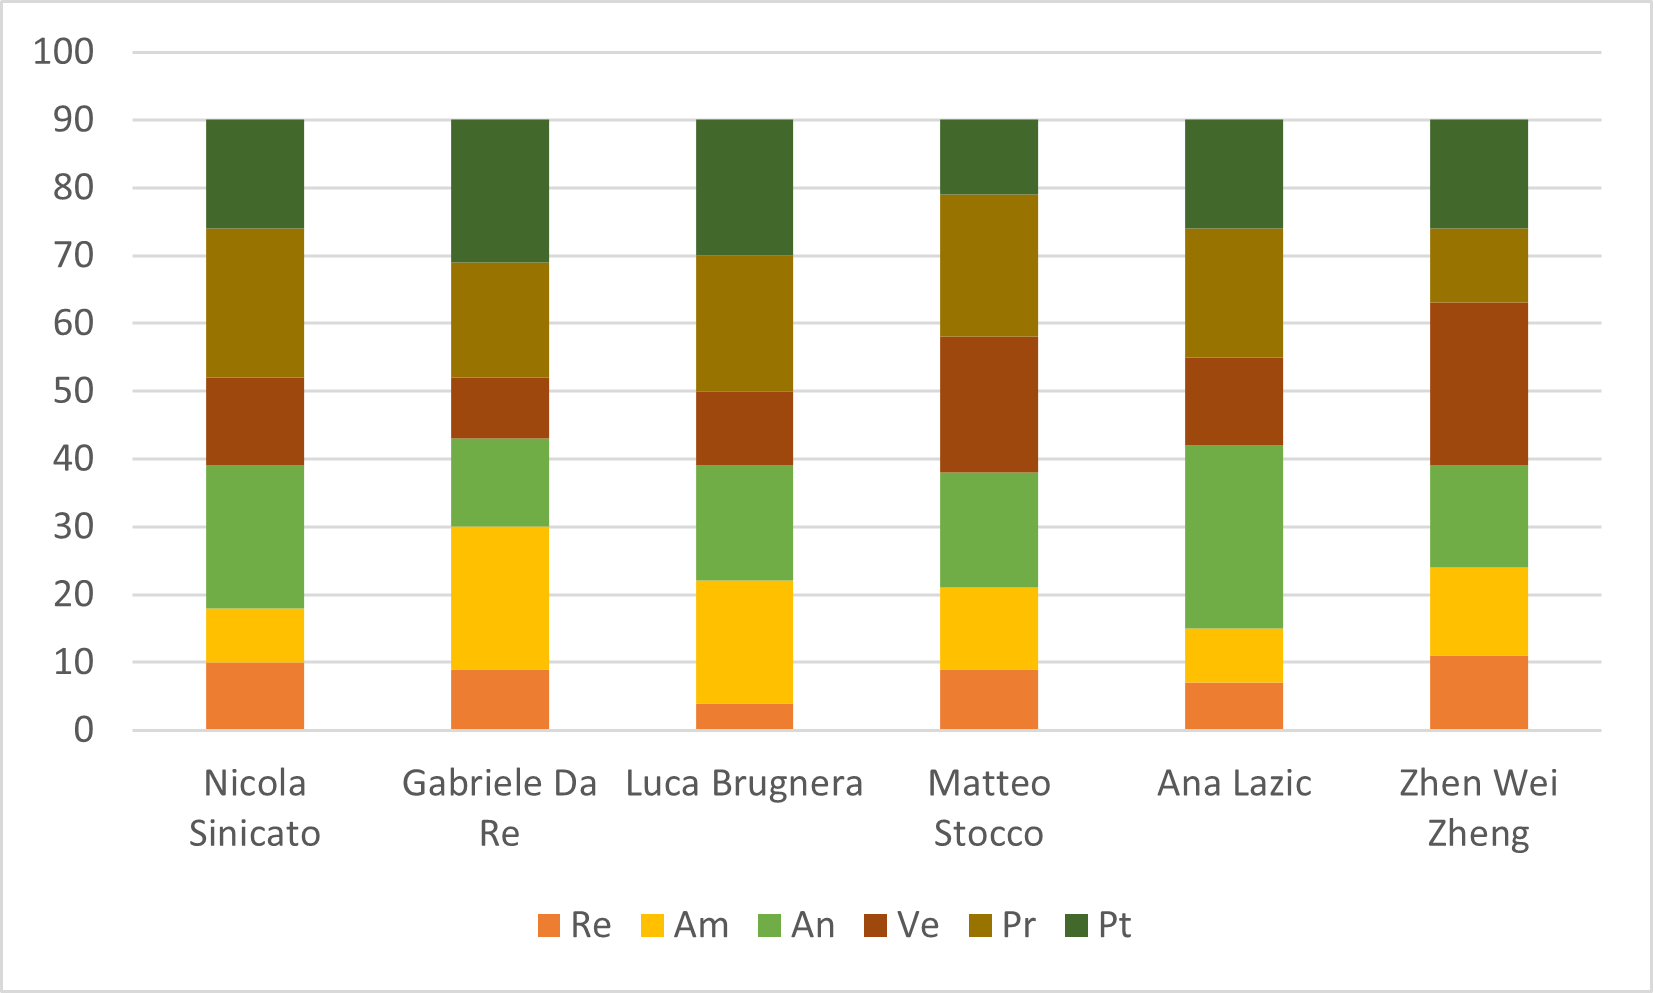
\includegraphics[scale=0.6]{img/grafi preventivo/istogrammi/totale/totale.png}
    \caption{Istogramma con la distribuzione oraria complessiva}
\end{figure}
\begin{figure}[H]
    \centering
    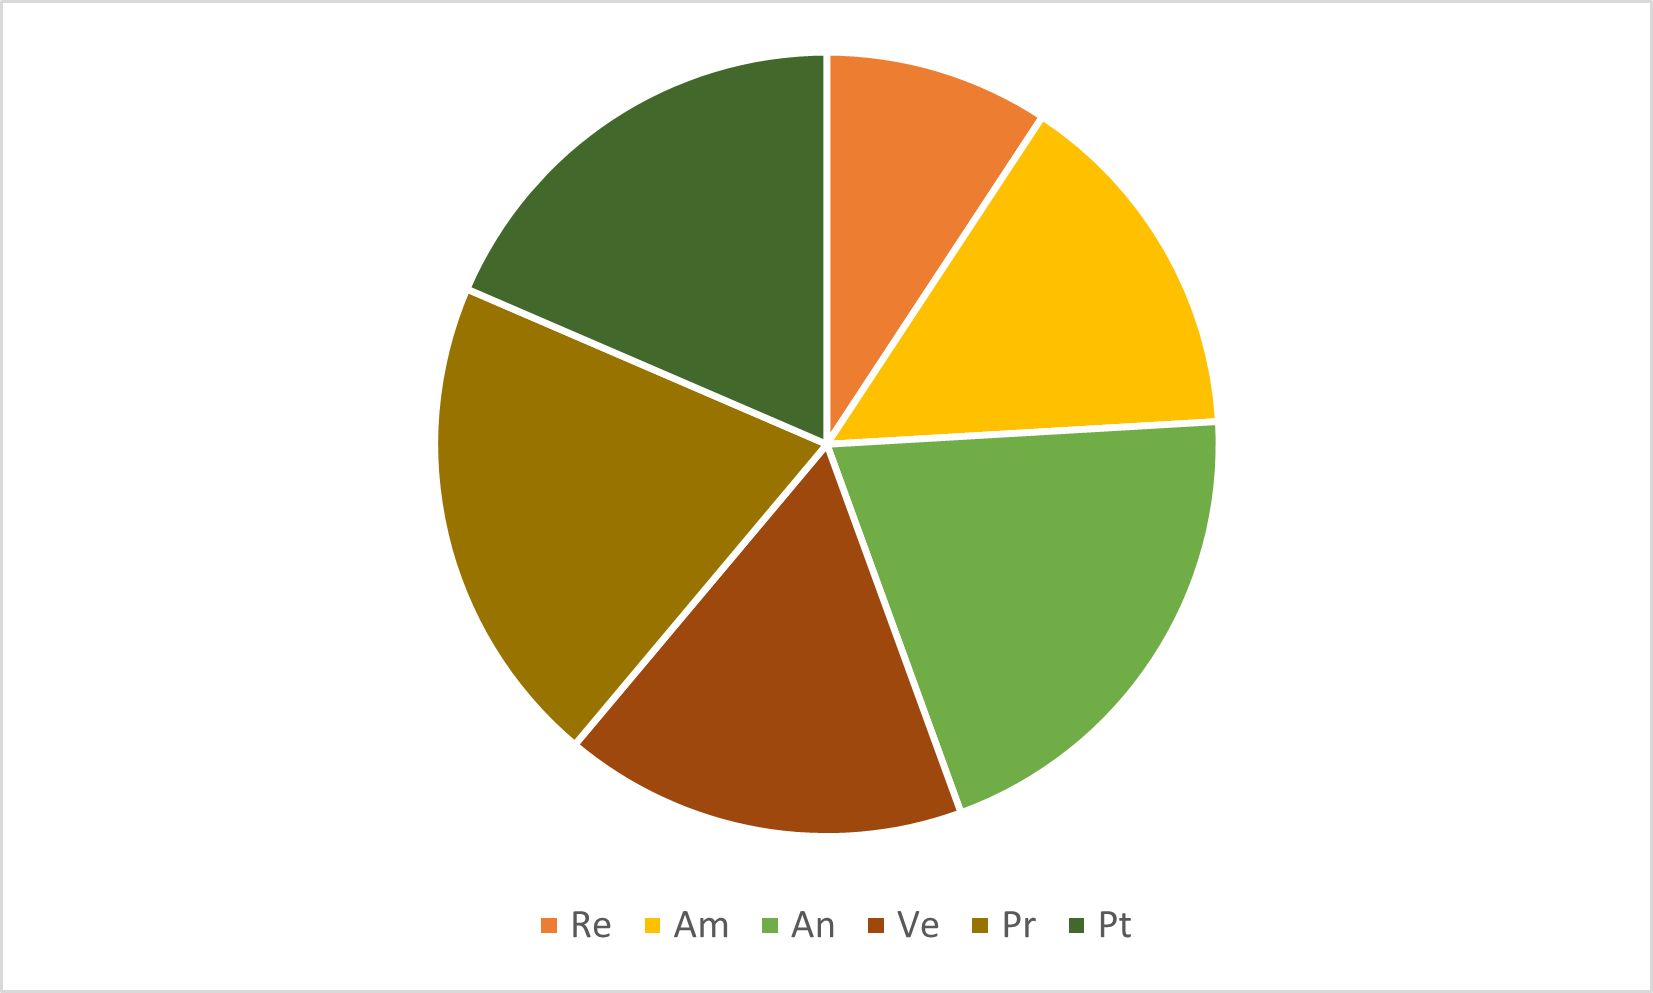
\includegraphics[scale=0.6]{img/grafi preventivo/torta/totale/totale.png}
    \caption{Grafico a torta con la ripartizione delle ore complessive per ruolo}
\end{figure}
\subsubsection{Preventivo dei costi}
La seguente tabella rappresenta le ore complessive dedicate ad ogni ruolo e il corrispettivo costo in euro:

	\setlength\extrarowheight{5pt}
	\rowcolors{2}{gray!10}{gray!40}
	\begin{tabularx}{\textwidth}{|ccc|c|}
		\hline
		\rowcolor{white}
		\textbf{Ruolo} & \textbf{Costo orario (€)} & \textbf{Ore totali} & \textbf{Costo totale (€)} \\
		\hline
		Responsabile &30&49&1470 \\
		Amministratore &20&85&1700 \\
		Analista &25&89&2225 \\
		Verificatore &15&138&2070 \\
		Programmatore &15&102&1530 \\
		Progettista &25&77&1925 \\
		\hline
		Totale &-&-&10920 \\
		\hline
		\rowcolor{white}
		\caption{Prospetto del costo orario per ruolo complessivo}
	\end{tabularx}
    \vspace{10pt}
	
% ----------------------------------------------------------------------------------------------------------------
